\chapter{Draft: Topology Optimization Approaches for the Curvature Minimization of Level Set Isocontours}
\label{sec:topology_optimization_approaches_for_the_curvature_minimization_of_level_set_isocontours}

% \documentclass[twocolumn]{svjour3}

% \smartqed

% \usepackage{fix-cm}
% \usepackage{graphicx}
% \usepackage{fixltx2e}
% \usepackage{dblfloatfix}
% \usepackage{subfig}
% \usepackage{tabularx}
% \usepackage{natbib}                        % Use citep, citet in citations
% \usepackage{amsmath,mathtools}             % Cases
% \usepackage{color}                         % Color text to indicate changes
% \usepackage{multirow}                      % More complex tables
% \usepackage{chngcntr}                      % Show section in table

% \counterwithout{table}{section}

% \journalname{Computational Mechanics}

% \begin{document}

% -----------------------------------------------------------------------------
% Title

% \title{Density and Level Set-XFEM Schemes for Topology Optimization of 3-D Structures}

% \subtitle{Topology Optimization in 3D}

% \author{Carlos H. Villanueva	\and Kurt Maute}

% \institute{
% 	C. H. Villanueva \at
% 	Department of Mechanical Engineering,\\
% 	University of Colorado at Boulder,\\
% 	Boulder, CO 427 UCB, USA\\
% 	e-mail: carlos.villanueva@colorado.edu\\
% 	\and
%	K. Maute \at
% 	Department of Aerospace Engineering,\\
% 	University of Colorado at Boulder,\\
% 	Boulder, CO 427 UCB, USA\\
% 	e-mail: maute@colorado.edu\\
% 	}

% \date{Received: date / Accepted: date}

% \maketitle

% -----------------------------------------------------------------------------
% Abstract

% \begin{abstract}

Curvature measures the smoothness of a surface. This paper studies the application of curvature minimization schemes to the zero level set isocontour. The objective is to maximize the smoothness of the level set surface of an optimized geometry. Rather than maximizing the smoothness of the surface using postprocessing methods like in \citep{LC:87}, the curvature minimization is inserted directly into the optimization problem.
% 
% \keywords{eXtended Finite Element Method \and Topology Optimization \and
% Solid Isotropic Material with Penalization \and Level Set Methods \and Additive Manufacturing \and 3D Printing}
% 
% \end{abstract}

% -----------------------------------------------------------------------------
% Introduction

% \section{Introduction}
% \label{sec:curvature_intro}

% -----------------------------------------------------------------------------

\section{Curvature}
\label{sec:curvature_methods}

Curvature is a mathematical concept that describes how sharply a curve bends; in other words, curvature measures how much a geometric object deviates from being flat. For example, the curvature of a straight line is identically zero, while curves that bend very little have small curvature and curves that bend sharply have large curvature.

The concept of curvature dates back to the Greek when Euclid provided a definition of the straight line as one which lies evenly with the points on itself; however, it was not until Newton that the concept of curvature was defined \citep{NC:1736}. As stated above, the basic idea is that some curves are straight, while some are curved. Among the different concepts behind curvature, they all agree that a circle has the same curvature at all the points of its circumference. Given that the smaller the radius, the greater the curvature, we can say that curvature is a quantity inversely proportional to the radius of the circle. Then, we can measure the curvature of any curve by measuring the curvature of the circle lying nearest to it \citep{Coolidge:52}.

A more formal definition of curvature states that if we move along a curve, the direction of the tangent vector will not change as long as the curve is flat. However, its direction will change if the curve bends. The more the curve bends, the more the direction of the tangent vector changes. Therefore, to study curvature we must study how the tangent vector changes as we move along a curve. But, because we are only interested in the direction of the tangent vector, not its magnitude, we will consider the unit tangent vector.

Let $C$ be a smooth curve with position vector $\mathbf{r}(s)$ where $s$ is the arc length parameter. The curvature $\kappa$ of $C$ is defined to be:
%
\begin{equation}
	\centering
	\label{eq:curvature_t}
	\kappa = \kappa_{t} = \Vert \frac{\mathrm{d} \mathbf{t}}{\mathrm{d}s} \Vert
\end{equation}
%
where $\mathbf{t}$ is the unit tangent vector.

Assuming the unit normal vector, $\mathbf{n}$ is orthonormal to the unit tangent vector, we can redefine curvature as:
%
\begin{equation}
	\centering
	\label{eq:curvature_n}
	\kappa = \kappa_{n} = \Vert \frac{\mathrm{d} \mathbf{n}}{\mathrm{d}s} \Vert
\end{equation}
%
Other definitions of curvature as a function of the normal unit vector can be found in \citep{WW:05,WW:04c,LLC+:08a}, where the mean curvature measure was used.
%
\begin{equation}
	\centering
	\label{eq:mean_curvature}
	H = \Vert \nabla \cdot \mathbf{n} \Vert
\end{equation}
%
% -----------------------------------------------------------------------------

\subsection{Comparison of curvature and mean curvature in $\mathbb{R}^2$}
\label{sec:comparison_curvature_mean_curvature}

Mathematically, Equations \ref{eq:mean_curvature} and \ref{eq:curvature_n} are equivalent for geometrical objects in $\mathbb{R}^2$. We will show this by computing the curvature and mean curvature of a circle in the examples below.

\subsubsection{Curvature of circle}
\label{sec:curvature_circle}

In this example, we will compute the curvature of a circle with radius $a$ to use as an analytical solution to our curvature measures of \ref{sec:numerical_sweeps}. We can parametrize the curve of the circle as a function of the arclength, $s$, as:
%
\begin{equation}
	\centering
	\label{eq:position_vector}
	\mathbf{r}\left( s \right) = \lbrace a\cos\frac{s}{a}, a\sin\frac{s}{a} \rbrace
\end{equation}
%
Then, the unit normal vector, $\mathbf{n}$, is defined as:
%
\begin{equation}
	\centering
	\label{eq:unit_normal_vector}
	\mathbf{n} \left( s \right) = \frac{\frac{\mathrm{d}\mathbf{r}}{\mathrm{d}s}}{\Vert \frac{\mathrm{d}\mathbf{r}}{\mathrm{d}s}\Vert}
\end{equation}
%
where $\frac{\mathrm{d}\mathbf{r}}{\mathrm{d}s}$ is computed as:
%
\begin{equation}
	\centering
	\label{eq:position_vector_derivative}
	\begin{split}
	\frac{\mathrm{d}\mathbf{r}}{\mathrm{d}s} & = \lbrace a \left( -\frac{1}{a} \sin\frac{s}{a} \right), a \left( \frac{1}{a} \cos\frac{s}{a} \right) \rbrace \\
	                                         & = \lbrace -\sin\frac{s}{a}, \cos\frac{s}{a} \rbrace
	\end{split}
\end{equation}
%
Thus, the unit normal vector, $\mathbf{n}$, is: 
%
\begin{equation}
	\centering
	\label{eq:unit_normal_vector_def}
	\mathbf{n} \left( s \right) = \lbrace - \sin \frac{s}{a}, \cos \frac{s}{a} \rbrace
\end{equation}
%
and its derivative with respect to the arclength is:
%
\begin{equation}
	\centering
	\label{eq:unit_normal_vector_derivative}
	\frac{\mathrm{d}\mathbf{n}}{\mathrm{d}s} = \lbrace -\frac{1}{a} \cos \frac{s}{a}, -\frac{1}{a} \sin \frac{s}{a} \rbrace
\end{equation}
%
Finally, the curvature $\kappa_{n}$ is:
%
\begin{equation}
	\centering
	\label{eq:curvature_solution}
	\kappa_{n} = \Vert \frac{\mathrm{d} \mathbf{n}}{\mathrm{d}s} \Vert = \frac{1}{a}
\end{equation}
%
We can conclude that the curvature of the circle is the inverse of its radius.

% -----------------------------------------------------------------------------

\subsubsection{Mean curvature of circle}
\label{sec:mean_curvature_circle}

Following the circle parametrization of Equation \ref{eq:position_vector}, we can compute the mean curvature (\ref{eq:mean_curvature}) of a circle as follows:
%
\begin{equation}
	\centering
	\label{eq:mean_curvature_definition}
	\begin{split}
	H & = \Vert \frac{\partial n_{x}}{\partial x} + \frac{\partial n_{y}}{\partial y} \Vert \\
	  & = \Vert \frac{\partial n_{x}}{\partial s} \frac{\partial s}{\partial x} + \frac{\partial n_{y}}{\partial s} \frac{\partial s}{\partial y} \Vert
	\end{split}
\end{equation}
%
From Equation \ref{eq:position_vector}, we parametrized $x$ as $a\cos\frac{s}{a}$ and $y$ as $a\sin\frac{s}{a}$. Therefore
%
\begin{equation}
	\centering
	\label{eq:partial_derivatives_s}
	\begin{split}
	\frac{\partial s}{\partial x} & = \frac{x}{\sqrt{x ^ 2 + y ^ 2}} = a \frac{\cos\frac{s}{a}}{a} \\
	\frac{\partial s}{\partial y} & = \frac{y}{\sqrt{x ^ 2 + y ^ 2}} = a \frac{\sin\frac{s}{a}}{a}	
	\end{split}
\end{equation}
%
From Equation \ref{eq:position_vector_derivative}, the derivative of the normal unit vector with respect to the arclength $s$ is:
%
\begin{equation}
	\centering
	\begin{split}
	\frac{\partial n_{x}}{\partial s} & = -\frac{1}{a} \cos \frac{s}{a} \\
	\frac{\partial n_{y}}{\partial s} & = -\frac{1}{a} \sin \frac{s}{a}
	\end{split}
\end{equation}
% 
Finally, the mean curvature is
%
\begin{equation}
	\centering
	\label{eq:mean_curvature_solution}
	H = \Vert -\frac{1}{a} \cos \frac{s}{a} \left( a \frac{\cos\frac{s}{a}}{a} \right) - \frac{1}{a} \sin \frac{s}{a} \left( a \frac{\sin\frac{s}{a}}{a} \right) \Vert = \frac{1}{a}
\end{equation}
%
We can conclude that the curvature \ref{eq:curvature_n} and mean curvature \ref{eq:mean_curvature} formulations are the same for a geometrical object in $\mathbb{R}^2$.

% -----------------------------------------------------------------------------

\subsubsection{Curvature of sinusoidal wave}
\label{sec:curvature_sinusoidal_wave}

This same methodology can be applied to compute the curvature of the sinusoidal wave:
%
\begin{equation}
	\centering
	\label{eq:parametric_sin_wave}
	\mathbf{r} \left( s \right) = \lbrace s, A \sin \pi s \rbrace
\end{equation}
%
where $A$ is the amplitude of the sinusoidal wave. The curvature is then:
%
\begin{equation}
	\centering
	\label{eq:sin_wave_curvature_solution}
	\kappa_{n} = \pi^2 \left(\frac{A^2 ( 1 + \cos{\left(\pi s\right)}^2 ) \sin{\left(\pi s\right)}^2}{{( 1 + A \pi \cos{\left(\pi s\right)}^2} ) ^ 3}\right)^2
\end{equation}

The results obtained in the numerical examples will be compared to these analytical formulations to attest the accuracy of our curvature measure.

Curvature and mean curvature are equivalent measures for geometrical objects in $\mathbb{R}^2$. Note, however, that this assertion is not applicable to three-dimensional objects.

% -----------------------------------------------------------------------------

\section{Curvature Squared}
\label{eq:curvature_squared}

\citep{DHK+:01,NTG+:14,OB:12} used the square power of the curvature $\kappa_{n}$ as their measurement formulation. Because the shape of interest is the zero level set isocontour, we will measure curvature in our design domain by integrating $\kappa_{n}^2$ over $\Gamma_{\phi=0}$.
%
\begin{equation}
	\centering
	\label{eq:curvature_integral}
	\int_{\phi=0} \kappa_{n}^2 \,\mathrm{d}\Gamma = \int_{\phi=0} \left(\Vert \frac{\mathrm{d}\mathbf{n}}{\mathrm{d}s} \Vert\right)^2 \,\mathrm{d}\Gamma
\end{equation}
%
% -----------------------------------------------------------------------------

\section{Level set normal unit vector}
\label{sec:normal_unit_vector}

As shown in section \ref{sec:curvature_methods}, we need to define the normal vector of the level set field in order to measure curvature along the $\Gamma_{\phi=0}$ isocontour. By definition of equation \ref{eq:level_set_regions}, we define the normal of the level set field as:
%
\begin{equation}
	\centering
	\label{eq:normal_unit_vector}
	\mathbf{n} = \frac{\nabla \phi}{\Vert \nabla \phi \Vert}
\end{equation}
%
For this curvature study, we will use several variations of the normal unit vector \ref{eq:normal_unit_vector} to compute the curvature.

% -----------------------------------------------------------------------------

\subsection{$\mathbf{n}_{\phi}$}
\label{sec:nphi}

Our first definition of a normal unit vector, which we will denote as $\mathbf{n}_{\phi}$, will enforce equation \ref{eq:normal_unit_vector} in a strong form:
%
\begin{equation}
	\centering
	\label{eq:normal_phi}
	\mathbf{n}_{\phi} = \frac{\nabla \phi}{\Vert \nabla \phi \Vert}
\end{equation}
%
The normal will be interpolated at the interface $\Gamma_{\phi=0}$ from the nodally defined level set field, using the elemental shape functions. Note that this formulation does not guarantee continuity of the level set normals at the nodes. For example, Figure \ref{fig:circle_physical_005} shows a circular inclusions of radius $0.05$ in a domain of size $3L \times 2L$, and Figure \ref{fig:circle_discrete_005} shows the discretized domain with $45 \times 30$ elements. Figure \ref{fig:circle_discrete_normals_005} zooms into the inclusion area and shows how the value of $\mathbf{n}_{\phi}$ at node is interpolated differently from each one of its four adjacent elements.
%
\begin{figure}
	\centering
	\begin{tabularx}{\linewidth}{XX}
		\subfloat[Physical model for a level set circular inclusion with a radius of $0.05$ in a domain of size $3L \times 2L$.]{
			\label{fig:circle_physical_005}
			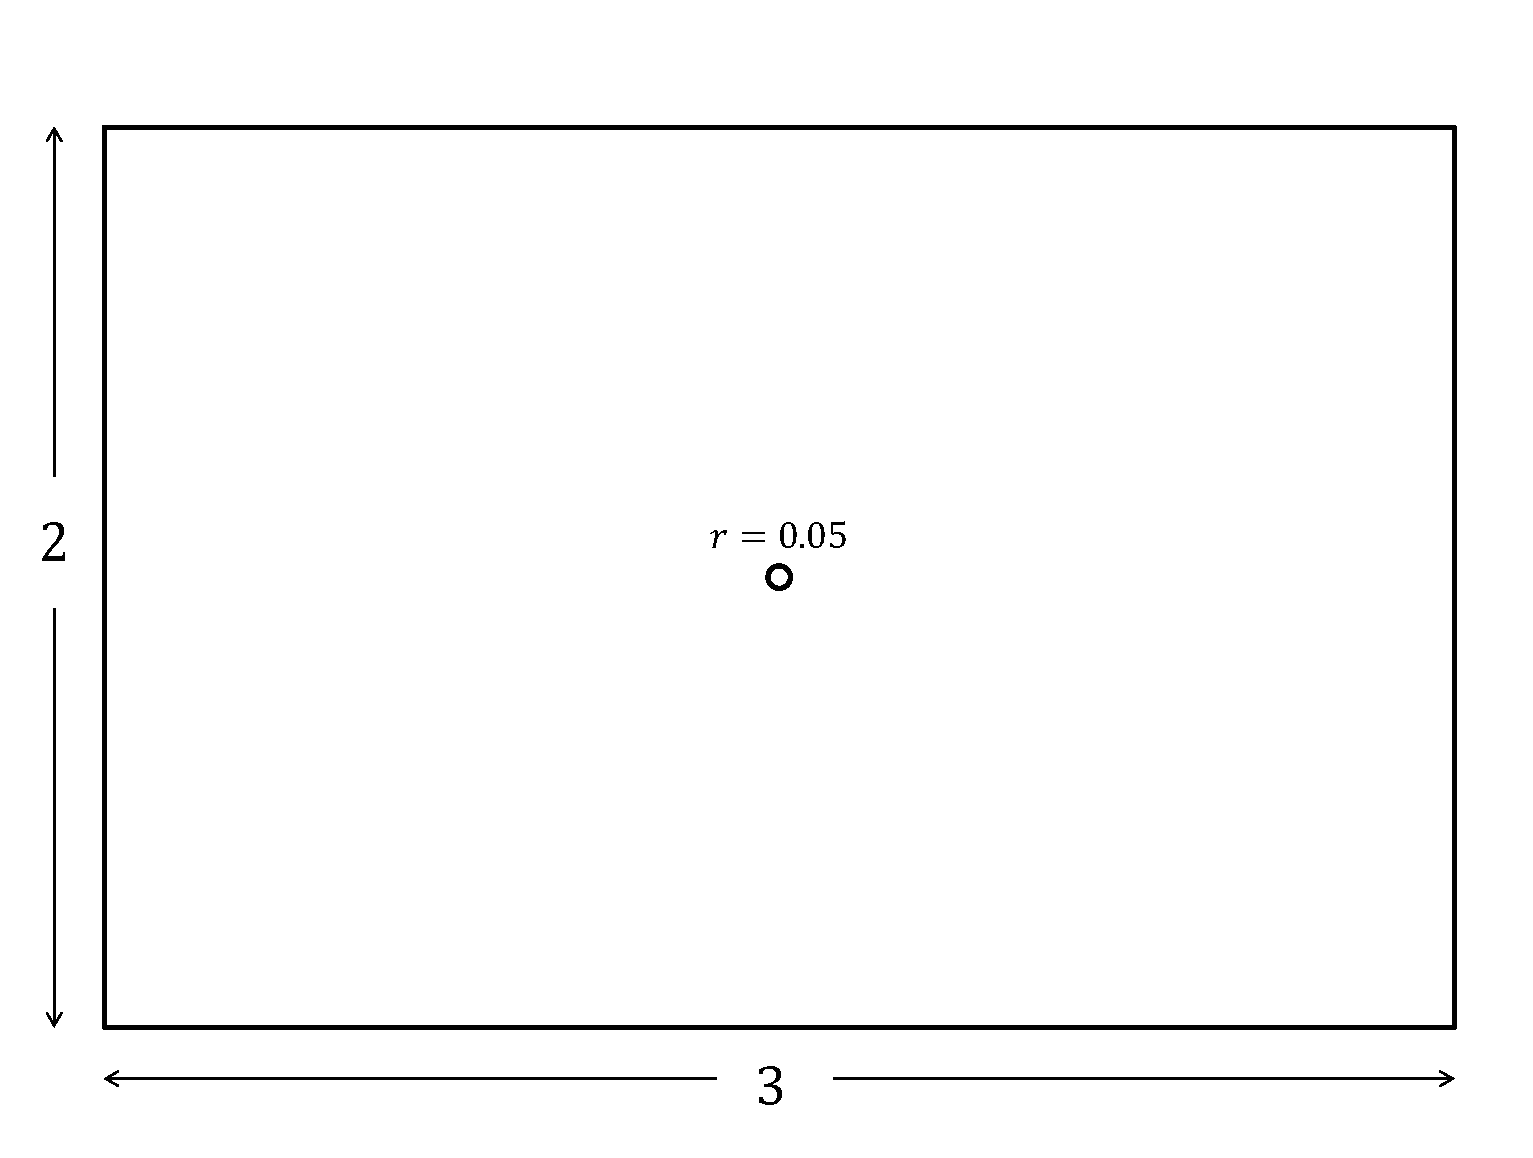
\includegraphics[width=\linewidth]{circle_physical_005.eps}
		} &
		\subfloat[Discrete model for a level set circular inclusion with a radius of $0.05$ in a domain with $45 \times 30$ elements. The red line indicates the location of $\Gamma_{\phi=0}$.]{
			\label{fig:circle_discrete_005}
			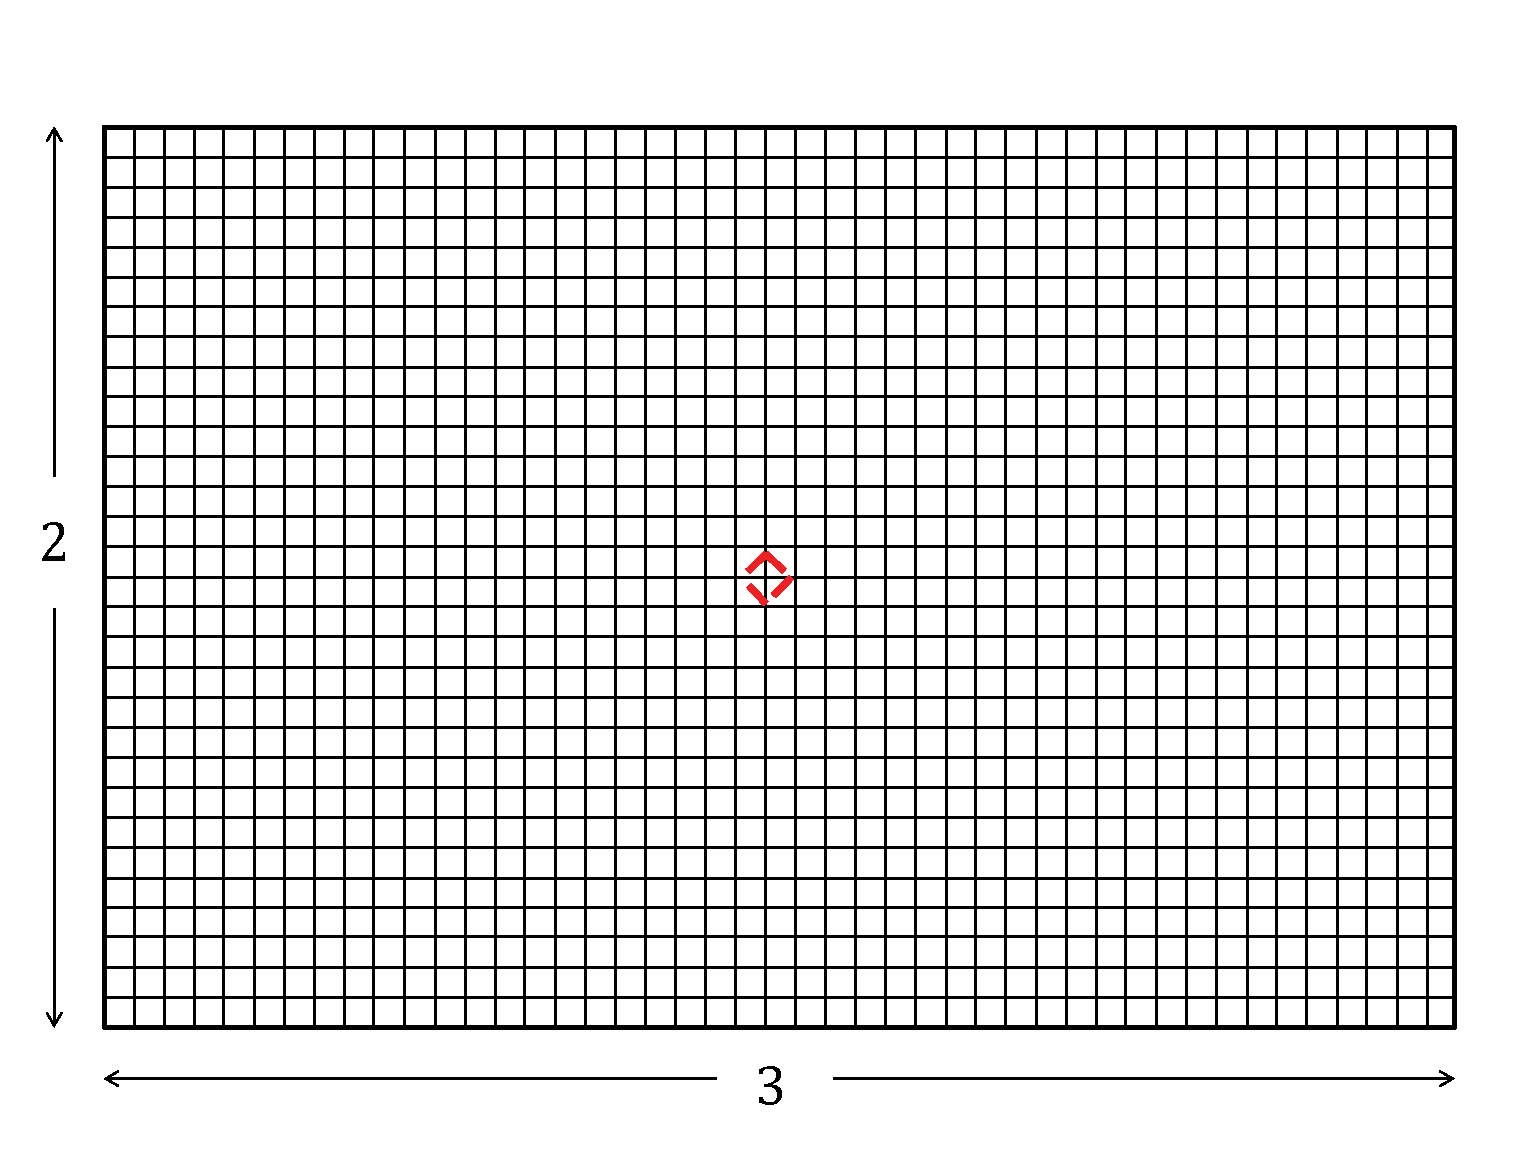
\includegraphics[width=\linewidth]{circle_discrete_005.eps}
		} \\
		\subfloat[$\mathbf{n}_{\phi}$ interpolated at a node from each of its four adjacent elements.]{
			\label{fig:circle_discrete_normals_005}
			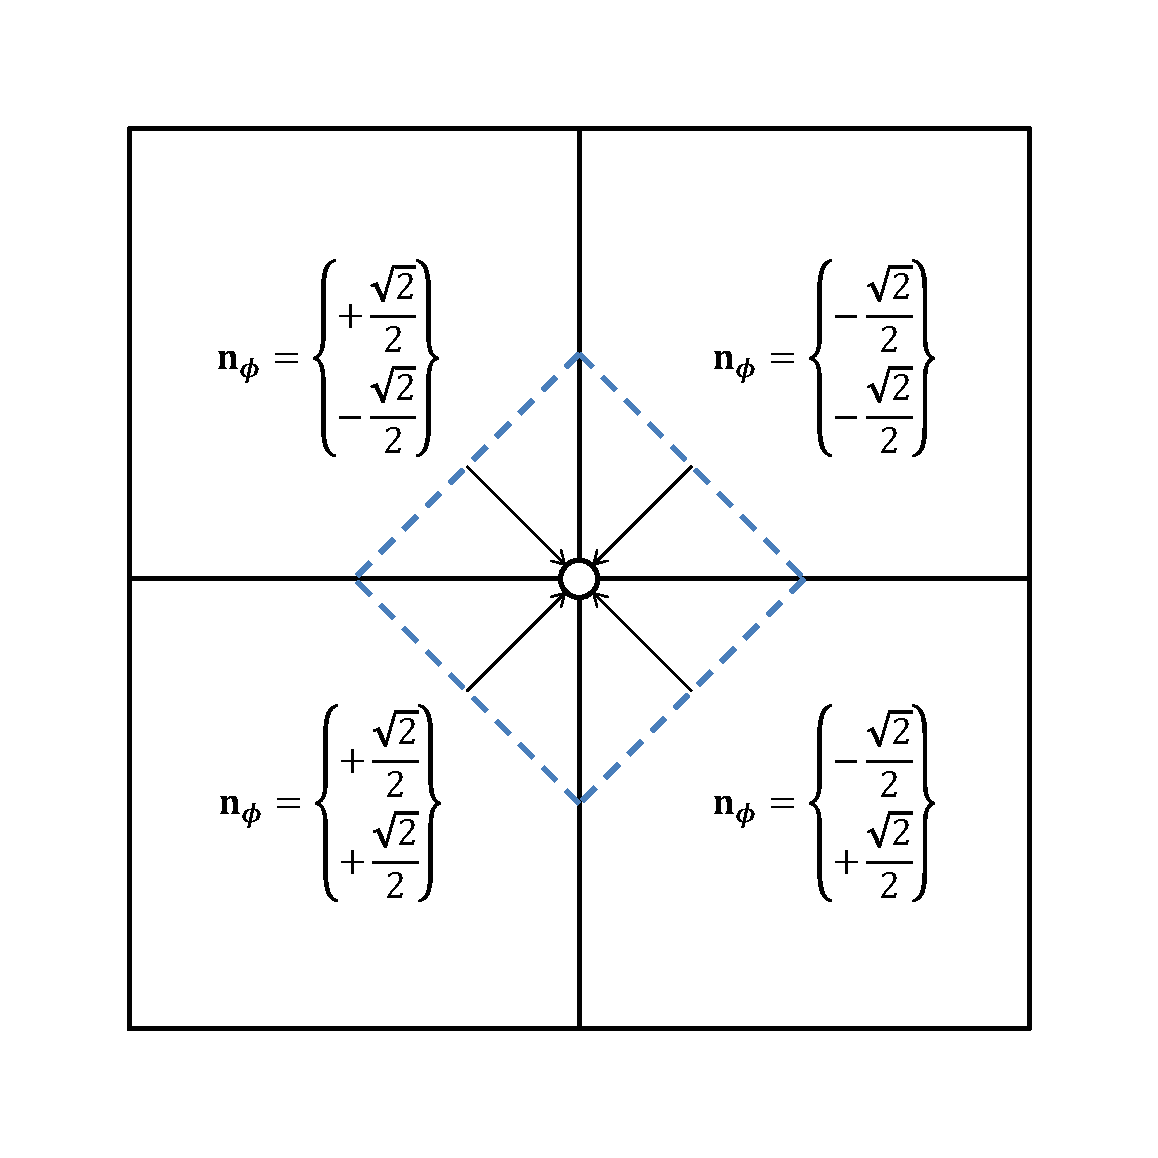
\includegraphics[width=\linewidth]{circle_discrete_normals_005.eps}
		}
	\end{tabularx}
	\caption{Discontinuities in the $\mathbf{n}_{\phi}$ field at a node.}
	\label{fig:nphi_discontinuities}
\end{figure}

% -----------------------------------------------------------------------------

\subsection{$\mathbf{n}_{u}$}
\label{sec:nnrm}

We will denote our second formulation as $\mathbf{n}_{u}$, and we will enforce Equation \ref{eq:normal_unit_vector} weakly:
%
\begin{equation}
	\centering
	\label{eq:normal_nrm}
	\int_{\Omega} \delta \mathbf{n}_{u} \left( \mathbf{n}_{u} \Vert \nabla \phi \Vert - \nabla \phi \right)\,\mathrm{d}\Omega = 0
\end{equation}
%
As our solution will be computed using the XFEM, we need to ensure continuity of the $\mathbf{n}_{u}$ degrees-of-freedom at the interface. We will impose a penalty formulation for the normal unit vector such that $\mathbf{n}_{u}^{+} = \mathbf{n}_{u}^{-}$ at $\Gamma_{\phi=0}$:
%
\begin{equation}
	\centering
	\label{eq:normal_nrm_interface}
	\begin{split}
	\gamma_{u} \int_{\Gamma^{+}} \delta \mathbf{n}_{u}^{+} \left( +\mathbf{n}_{u}^{+} - \mathbf{n}_{u}^{-} \right)\,\mathrm{d}\Gamma^{+} = 0 \\
	\gamma_{u} \int_{\Gamma^{-}} \delta \mathbf{n}_{u}^{-} \left( -\mathbf{n}_{u}^{+} + \mathbf{n}_{u}^{-}  \right)\,\mathrm{d}\Gamma^{-} = 0
	\end{split}
\end{equation}
%
where $\gamma_{u}$ is a scaling factor. Equation \ref{eq:normal_phi} is computed locally at the element level and does not ensure a continuous normal unit vector field at the nodes, as shown in Figure \ref{fig:nphi_discontinuities}. This alternative formulation, \ref{eq:normal_nrm}, seeks to study the effect on the curvature measure of using a continuous field.

% -----------------------------------------------------------------------------

\subsection{$\mathbf{n}_{\psi}$}
\label{sec:npsi}

Our last formulation with regards to the level set normal unit vector will be similar to Equation \ref{eq:normal_nrm_interface}. However, this formulation will first project the level set field using a smooth Heaviside function. For this goal, we will use the hyperbolic tangent function introduced by \citep{OK:05} and \citep{OKZ:07}:
%
\begin{equation}
	\centering
	\label{eq:smooth_heaviside_level_set}
	\psi\left( \phi \right) = \frac{1}{2} \left( \tanh \left( \frac{\phi}{2\epsilon} \right) + 1 \right)
\end{equation}
%
where $\epsilon$ determines the thickness of the profile. By using this projection, the interface is no longer defined by the $\phi = 0$ isocontour, but rather by $\psi = 0.5$. Figure \ref{fig:phi_to_psi_projection} shows the original level set function and their hyperbolic tangent projection for different values of $\epsilon$.
%
\begin{figure}
	\centering
	\begin{tabularx}{\linewidth}{XX}
		\subfloat[$\phi$]{
			\label{fig:phi_circle}
			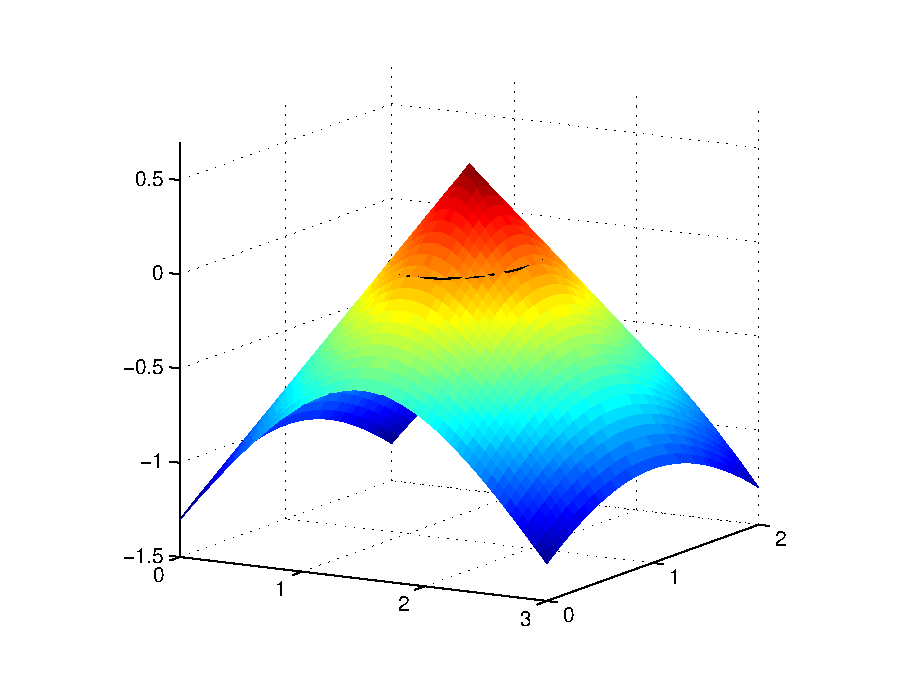
\includegraphics[width=\linewidth]{phi_circle.eps}
		} &
		\subfloat[$\epsilon=1.0$.]{
			\label{fig:psi_circle_epsilon_1}
			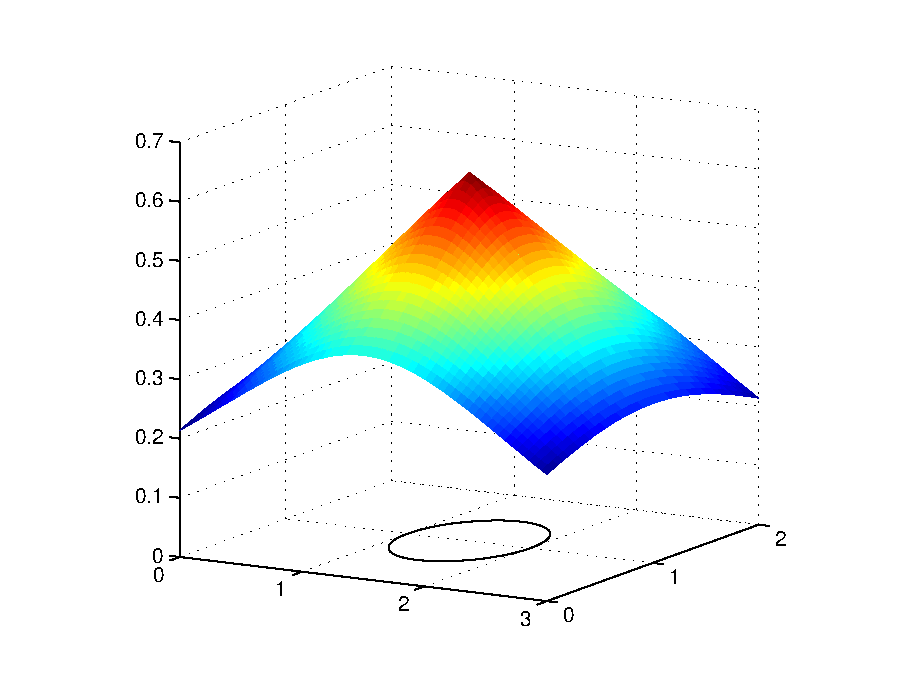
\includegraphics[width=\linewidth]{psi_circle_epsilon_1.eps}
		} \\
		\subfloat[$\epsilon=2.0$.]{
			\label{fig:psi_circle_epsilon_2}
			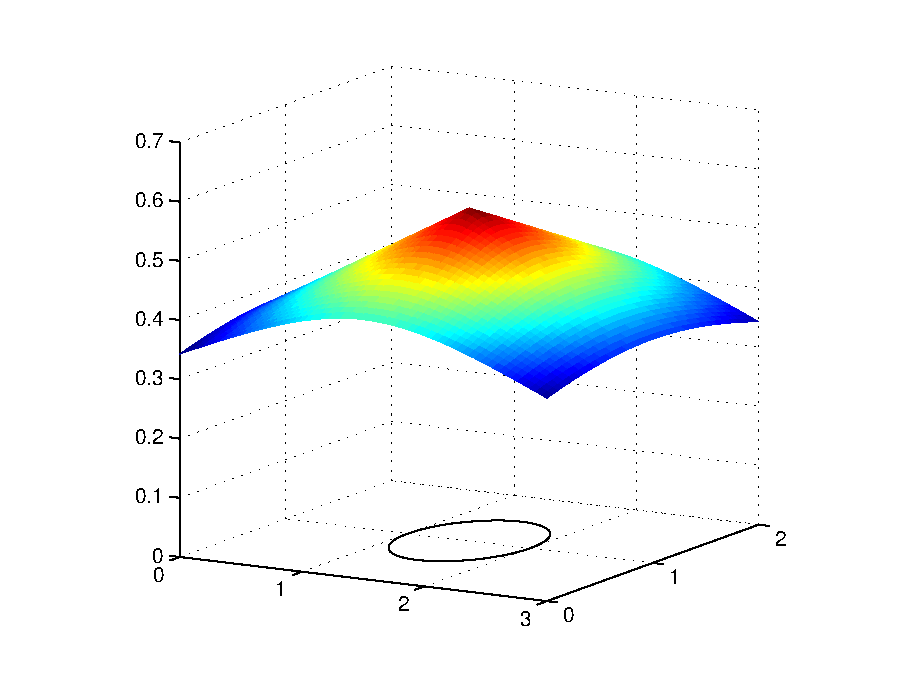
\includegraphics[width=\linewidth]{psi_circle_epsilon_2.eps}
		} &
		\subfloat[$\epsilon=4.0$.]{
			\label{fig:psi_circle_epsilon_4}
			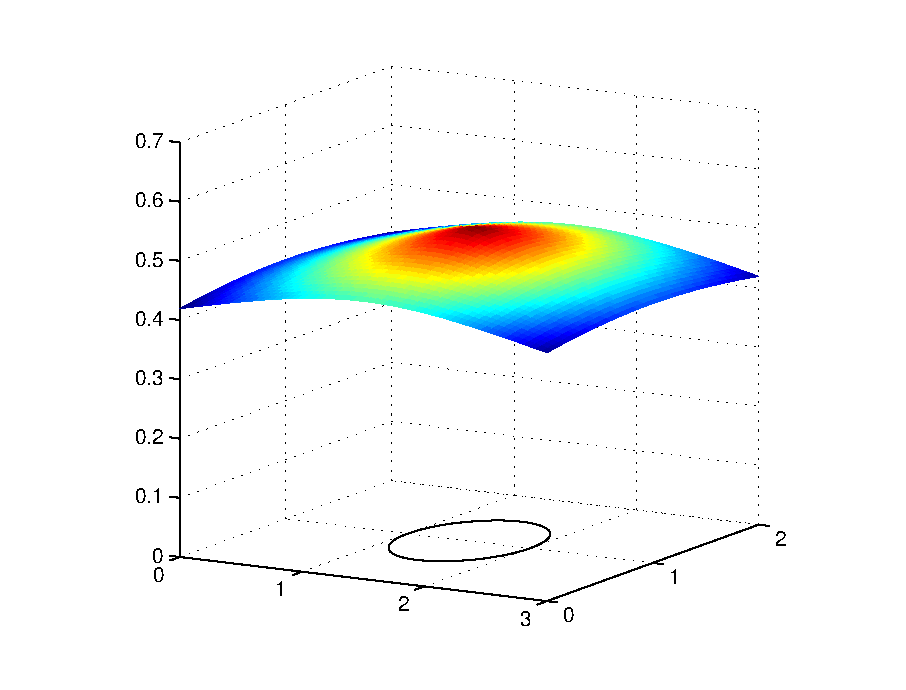
\includegraphics[width=\linewidth]{psi_circle_epsilon_4.eps}
		}
	\end{tabularx}
	\caption{A level set field for a circular inclusion of radius $0.5$, and their respective hyperbolic tangent projections for different values of $\epsilon$.}
	\label{fig:phi_to_psi_projection}
\end{figure}
%
The new weak form looks as follows:
%
\begin{equation}
	\centering
	\label{eq:normal_psi}
	\int_{\Omega} \delta \mathbf{n}_{\psi} \left( \mathbf{n}_{\psi} \Vert \nabla \psi \Vert - \nabla \psi \right)\,\mathrm{d}\Omega = 0
\end{equation}
%
with interface conditions:
%
\begin{equation}
	\centering
	\label{eq:normal_psi_interface}
	\begin{split}
	\gamma_{\psi} \int_{\Gamma^{+}} \delta \mathbf{n}_{\psi}^{+} \left( +\mathbf{n}_{\psi}^{+} - \mathbf{n}_{\psi}^{-} \right)\,\mathrm{d}\Gamma^{+} = 0 \\
	\gamma_{\psi} \int_{\Gamma^{-}} \delta \mathbf{n}_{\psi}^{-} \left( -\mathbf{n}_{\psi}^{+} + \mathbf{n}_{\psi}^{-}  \right)\,\mathrm{d}\Gamma^{-} = 0
	\end{split}
\end{equation}
%
where $\gamma_{\psi}$ is the scaling factor.

There are two ways to compute $\nabla \psi$ for Equation \ref{eq:normal_psi}. The first approach will compute $\psi\left(\phi\right)$ at the nodes and then use the element shape functions to interpolate to the integration point as:
%
\begin{equation}
	\centering
	\label{eq:nabla_psi_nodal}
	\nabla \psi = \frac{\partial \psi}{\partial \mathbf{x}}
\end{equation} 

Our second approach will first interpolate the $\phi$ field, and then apply chain rule to get $\nabla \psi$ as:
%
\begin{equation}
	\centering
	\label{eq:nabla_psi_gauss}
	\nabla \psi = \frac{\partial \psi}{\partial \phi} \frac{\partial \phi}{\partial \mathbf{x}}
\end{equation} 

where $\frac{\partial \psi}{\partial \phi}$ is computed analytically. To differentiate between the two approaches, we will refer to the first formulation as $\mathbf{n}_{\psi_{\phi}}$, and $\mathbf{n}_{\psi_{\mathrm{gp}}}$ for the second.

% -----------------------------------------------------------------------------

\subsection{$\mathbf{n}_{g}$}
\label{sec:ngeo}

The final formulation will consider the interface of the cut elements as geometrical objects, and compute the normal unit vector $\mathbf{n}_{g}$ from the coordinates of these objects. This approach will not be used with Equation \ref{eq:curvature_squared}, but rather to an equivalent formulation by measuring strain energy.

The square power of the curvature is an equivalent measure to strain energy. The use of $\mathbf{n}_{g}$ allows us to model the level set interface as a set of structural linear beam elements, and can solve a finite element problem and compute the strain energy of the system. Our measure of curvature squared is then:
%
\begin{equation}
	\centering
	\label{eq:curvature_strain_energy}
	\int_{\phi=0} \kappa_{n}^{2} \,\mathrm{d}\Gamma = \frac{1}{2} \int_{\phi=0} \boldsymbol{\sigma} : \boldsymbol{\varepsilon} \,\mathrm{d}\Gamma
\end{equation}
%
\begin{figure}
	\centering
	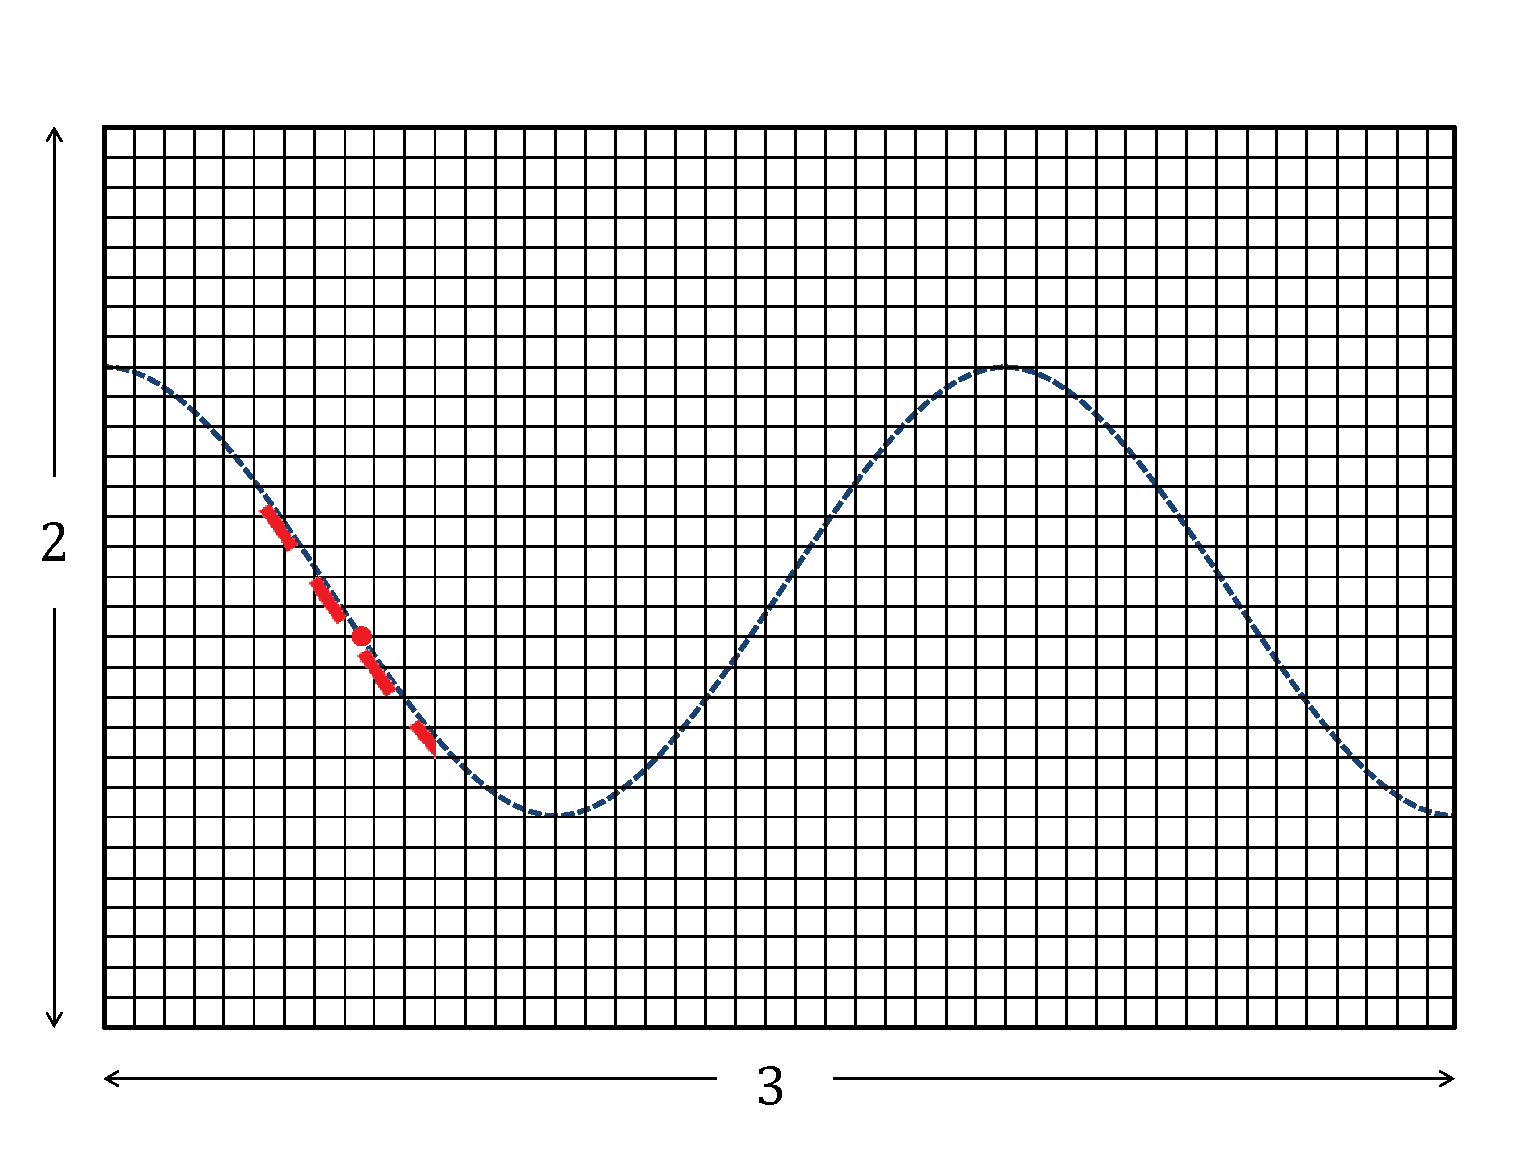
\includegraphics[scale=0.4]{beam_setup.eps}
	\caption{Sinusoidal wave with an amplitude of $0.50$. Mesh discretization is $45 \times 30$ elements. The red dot indicates one of the points at which the level set function intersects an element. The red dotted line indicates all cut elements that lie on the same interface of the red dot within a search radius $r_{\kappa} = 0.4$.}
	\label{fig:beam_setup}
\end{figure}
%
To illustrate the application of this approach, consider a level set function that describes a sinusoidal wave \ref{eq:level_set_sin_wave} with an amplitude $A_{s}$ of 0.50, as shown in Figure \ref{fig:beam_setup}. The red dot in the figure indicates one of the many points at which the level set function intersects an element. To compute the strain energy at this location, we define a search radius $r_{\kappa}$, and look for all the cut elements that share the same interface and that are within distance of this radius, as shown in Figure \ref{fig:beam_setup_zoom}. From these elements, we extract the interfaces and build a set of structural linear beam elements, as shown in Figure \ref{fig:beam_setup_elements}. The beam elements are assumed to be at rest; therefore, the initial displacements for $u_{x}$ and $u_{y}$ are equal to zero. For all internal nodes, we define two rotational degrees-of-freedom, one for each element connected to a node. End nodes only have a single rotational degree-of-freedom, as shown in Figure \ref{fig:beam_setup_elements}. We assume the rotations at the internal nodes are continuous:
%
\begin{figure}
	\centering
	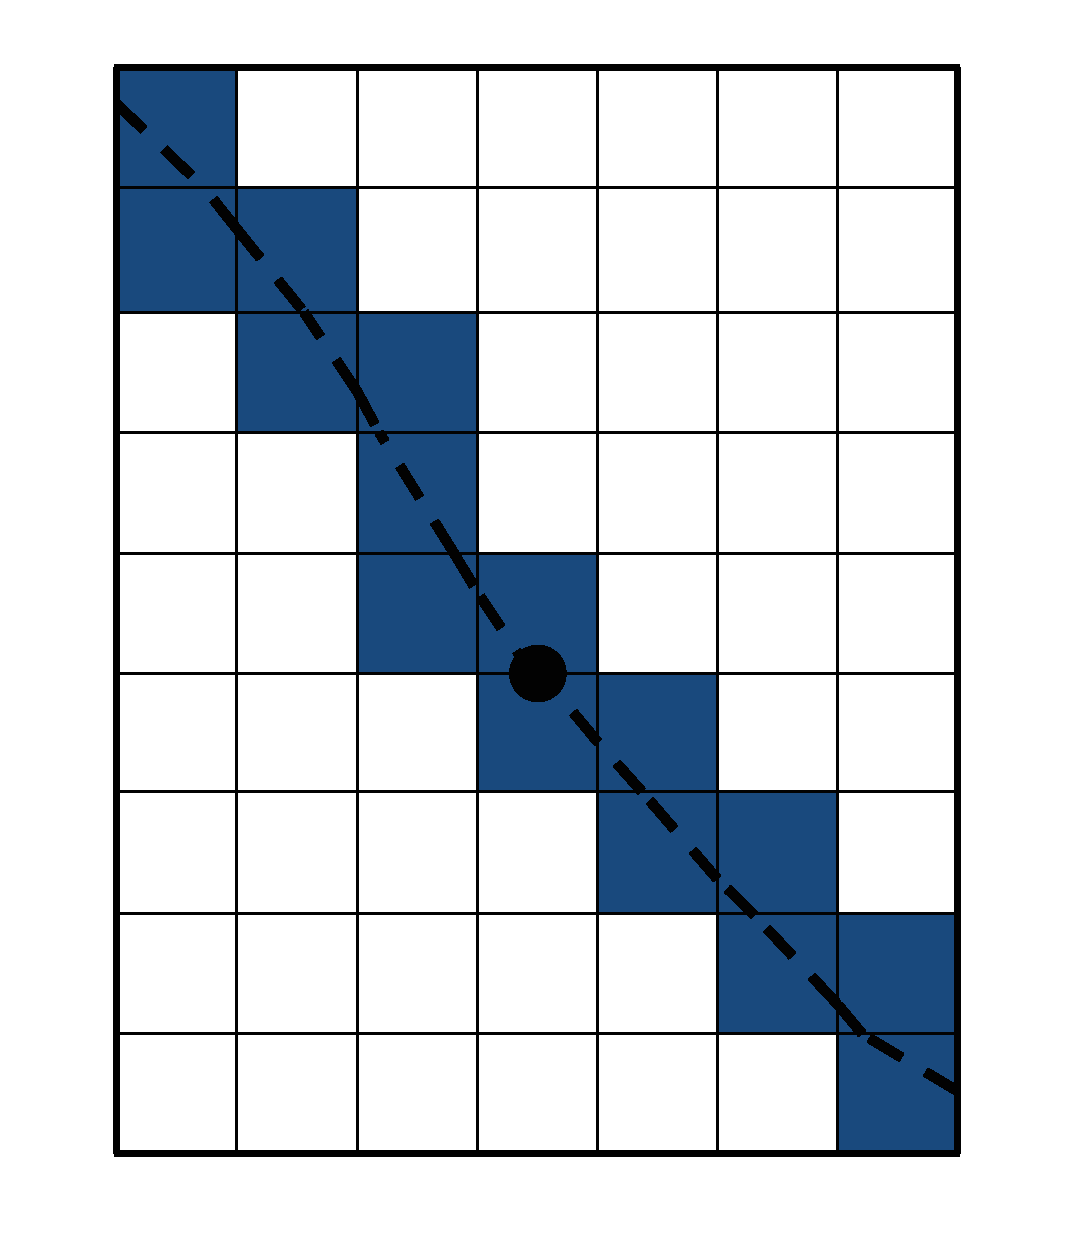
\includegraphics[scale=0.5]{beam_setup_zoom.eps}
	\caption{Zoomed image for the cut elements within the search radius $r_{\kappa} = 0.4$. Blue elements represent the cut element that are on the same interface.}
	\label{fig:beam_setup_zoom}
\end{figure}
%
\begin{equation}
	\centering
	\label{eq:continuous_rotation}
	\theta^{L}_{z} - \theta^{R}_{z} = \alpha_{CR}
\end{equation}
%
where $\theta^{L}_{z}$ is the rotation of the left adjacent element around the $z$ axis, $\theta^{R}_{z}$ is the rotation of the right one, and $\alpha_{CR}$ is computed for every node as a function of the geometrical normal of its adjacent elements, as shown in Figure \ref{fig:beam_setup_angle}:
%
\begin{equation}
	\centering
	\begin{split}
	\mathbf{n}_{g}^{C}  = \frac{\mathbf{n}_{g}^{L} + \mathbf{n}_{g}^{R}}{2} \\
	\mathbf{n}_{g}^{LC} = \mathbf{n}_{g}^{L} \times \mathbf{n}_{g}^{C} \\
	\mathbf{n}_{g}^{CR} = \mathbf{n}_{g}^{C} \times \mathbf{n}_{g}^{R} \\
	\alpha_{CR} = \frac{{\mathbf{n}_{g}^{LC}}_{z}}{\sqrt{1 - {{\mathbf{n}_{g}^{LC}}_{z}}^{2}}} + \frac{{\mathbf{n}_{g}^{CR}}_{z}}{\sqrt{1 - {{\mathbf{n}_{g}^{CR}}_{z}}^{2}}}
	\end{split}
\end{equation}
%
\begin{figure}
	\centering
	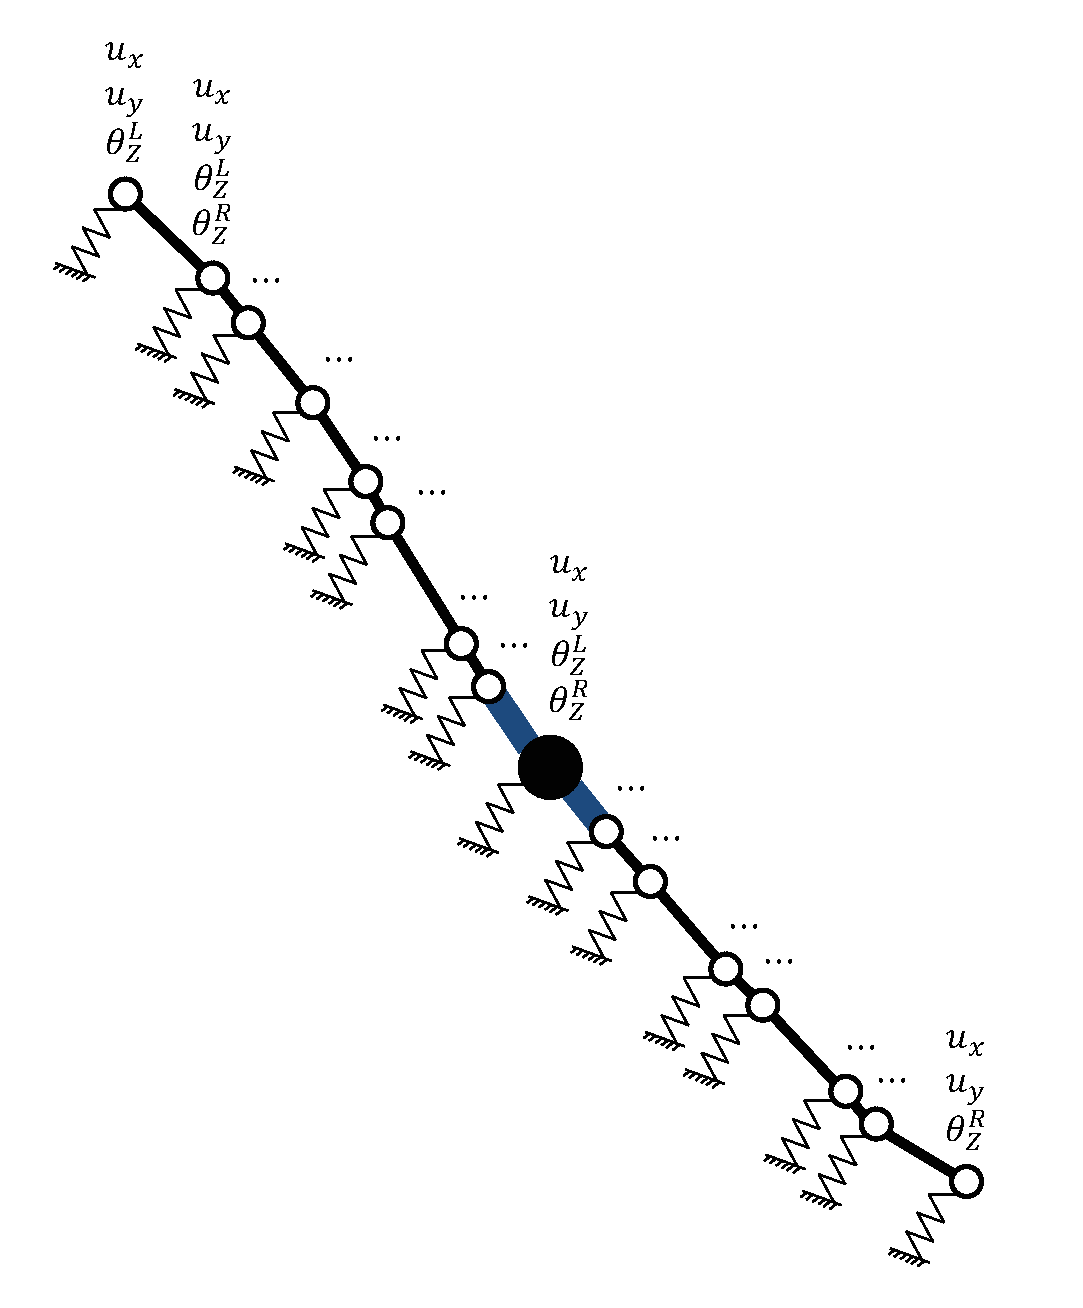
\includegraphics[scale=0.6]{beam_setup_elements.eps}
	\caption{Discretization of the structural linear beam elements. Inner nodes have two separate rotational degrees-of-freedom, left and right, one for each adjacent element. Nodes at the end of the interface only have a single rotational degree-of-freedom. All nodes rest on a field of artificial springs.}
	\label{fig:beam_setup_elements}
\end{figure}
%
The finite element problem solves for the displacement and rotational degrees-of-freedom, and the Lagrange multipliers. Despite the fact that the finite element problem consists of multiple elements, the strain energy of the point of interest is only computed on the adjacent elements as:
%
\begin{equation}
	\centering
	\label{eq:strain_energy_adjacent}
	\Pi^{C} = \frac{1}{2}\left(\Pi^{L} + \Pi^{R}\right)
\end{equation}
%
\begin{figure}
	\centering
	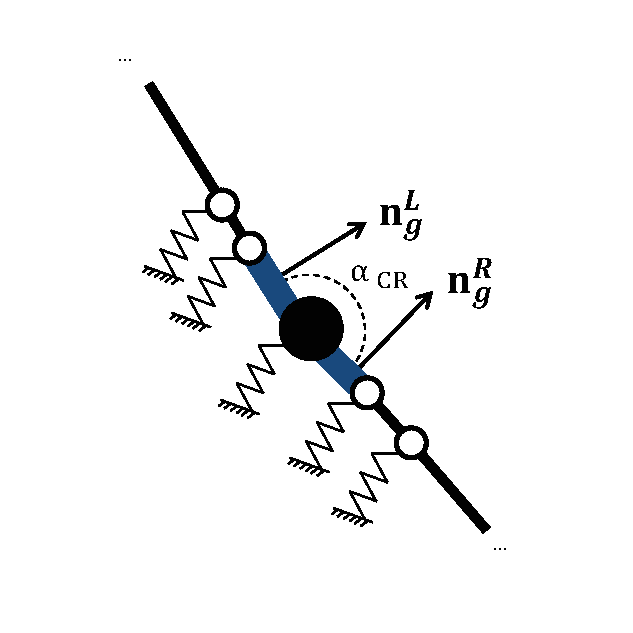
\includegraphics[scale=0.75]{beam_setup_angle.eps}
	\caption{Computation of $\alpha_{\mathrm{CR}}$. $\alpha_{\mathrm{CR}}$ is a function of the geometrical normal unit vectors of the adjacent elements.}
	\label{fig:beam_setup_angle}
\end{figure}
%
where $\Pi^{C}$ is the strain energy of the intersection point. The reason for this approach is that a larger number of elements yield a more accurate description of the rotations at the point of interest; however, once we get the solution, we are only interested in the strain energy of the adjacent elements because we will perform this procedure for all intersection points in the domain.

Initial computations showed that the strain energy of the system is highly sensitive to the discretization of the level set function. If the projection of a point in the function onto the mesh is off by a small amount due to discretization errors, it leads to large changes in the computed curvature when compared to its analytical value. To ameliorate this issue, we introduce a field of artificial springs with stiffness coefficient $k_{\kappa}$ to allow the points to move to what their correct location should be given the enforcement of the rotations, as shown in Figure \ref{fig:beam_setup_elements}.

% -----------------------------------------------------------------------------
% Numerical sweeps

\section{Methodology}
\label{sec:numerical_sweeps}

The squared curvature of two geometrical objects, a circle and a sinusoidal wave, will be studied. The objective of this study is to find the accuracy of our curvature measure by comparing the results to the analytical solutions we obtained in Section \ref{sec:curvature_circle}. We will use the results of this section to select the most promising approaches and later minimize the curvature of the level set interface.

% -----------------------------------------------------------------------------

\subsection{Sweep setup}
\label{sec:sweep_setup}

For our circle sweep, we will model the level set field with the following equation:
%
\begin{equation}
	\centering
	\label{eq:level_set_circle}
	\phi_{i} = r_{c} - \sqrt{x_{i} ^ 2 + y_{i} ^ 2}
\end{equation}
%
where $\phi_{i}$ represents a level set value at a node, and $x_{i}$ and $y_{i}$ are the spatial coordinates. We will vary the radius of the circle $r_{c}$ from a value of $0.25$ to $0.95$ in $100$ steps , as shown in Figure \ref{fig:circle_sweep_setup}. From Equations \ref{eq:curvature_solution} and \ref{eq:curvature_integral}, the curvature will be equal to:
%
\begin{equation}
	\centering
	\label{eq:curvature_analytical_circle}
	\int_{\phi=0} \kappa_{n}^2 \,\mathrm{d}\Gamma = \frac{2\pi}{r_{c}}
\end{equation}
%
\begin{figure}[H]
	\centering
	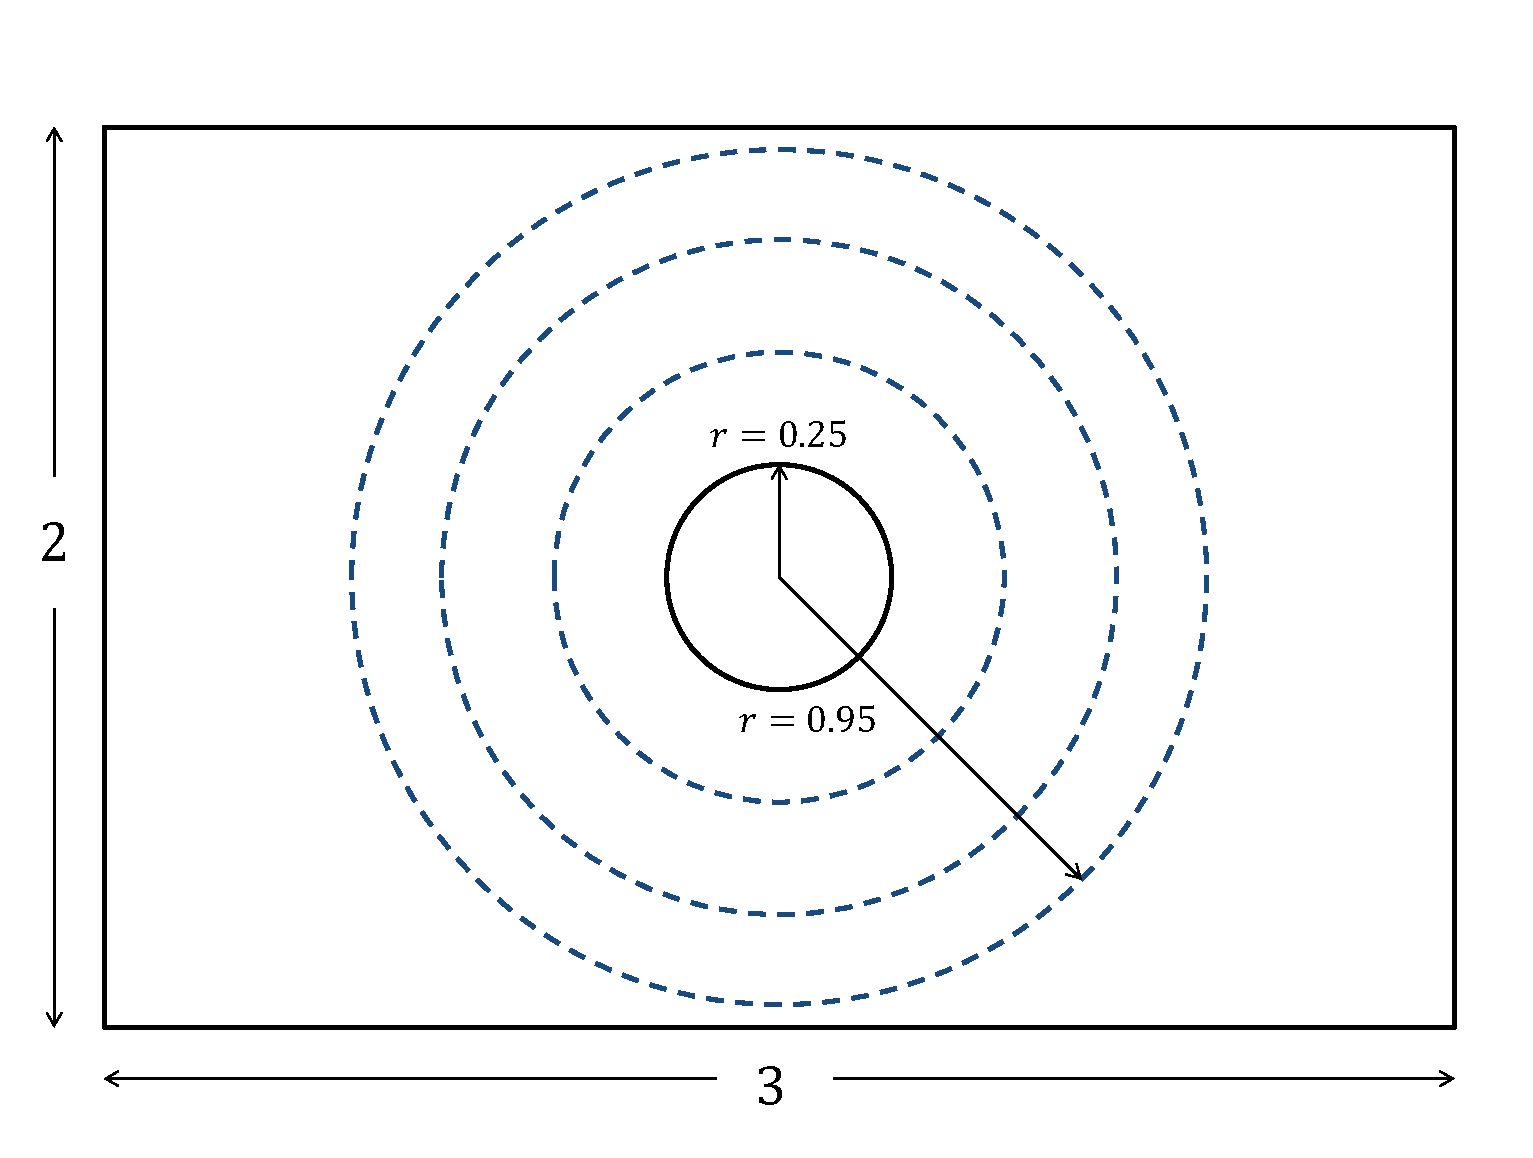
\includegraphics[scale=0.4]{circle_sweep_setup.eps}
	\caption{Setup for sweeping over the radius of a circle ranging from $0.25$ to $0.95$.}
	\label{fig:circle_sweep_setup}
\end{figure}

The sinusoidal wave will be modeled by the following equation:
%
\begin{equation}
	\centering
	\label{eq:level_set_sin_wave}
	\phi_{i} = y_{i} - A_{s} \sin \pi x_{i}
\end{equation}
%
where we will sweep over the amplitude of the sinusoidal wave, $A_{s}$, from $0.25$ to $0.75$, as shown in Figure \ref{eq:level_set_sin_wave}.
%
\begin{figure}[H]
	\centering
	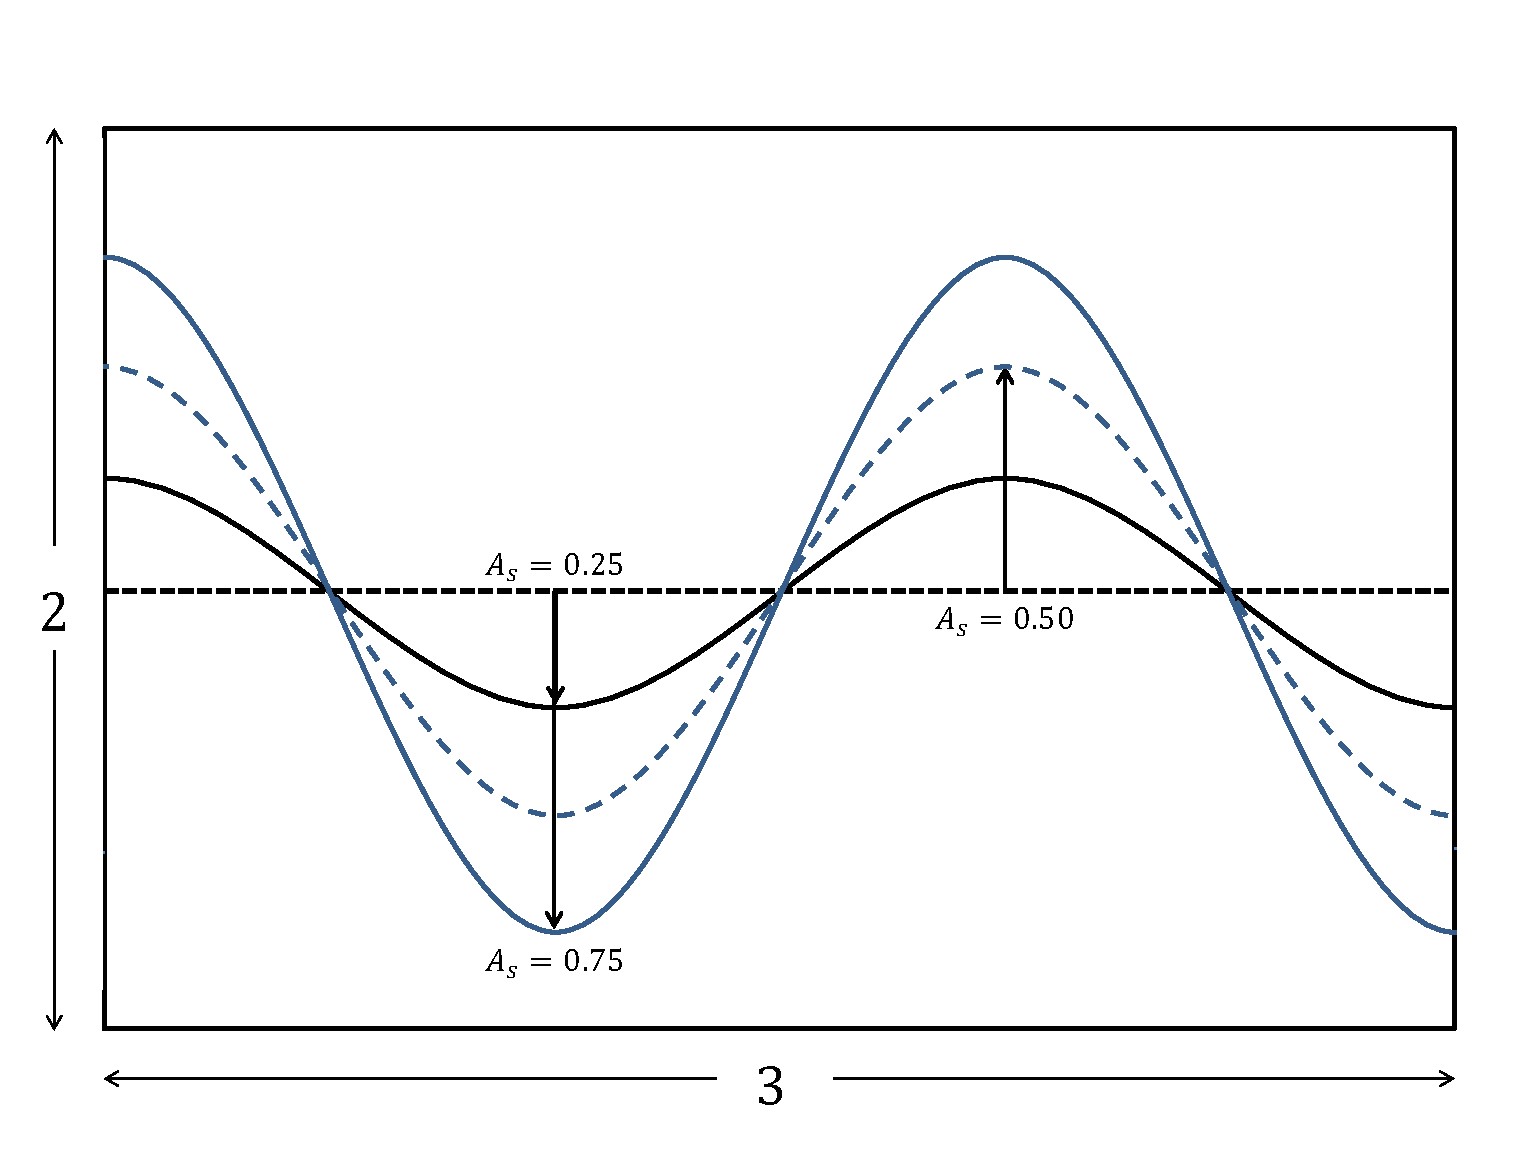
\includegraphics[scale=0.4]{sin_wave_sweep_setup.eps}
	\caption{Setup for sweeping over the amplitude of a sinusoidal wave ranging from $0.25$ to $0.75$.}
	\label{fig:sin_wave_sweep_setup}
\end{figure}
%
The mesh has spatial dimensions of $3L \times 2L$, and will be divided into $45 \times 30$ elements. The finer version of the mesh will have $180 \times 120$ elements.

% -----------------------------------------------------------------------------

\subsection{Preliminary sweep results}
\label{sec:sweep_results}

% -----------------------------------------------------------------------------

\subsubsection{$\mathbf{n}_{\phi}$ results}
\label{sec:nphi_results}

The results for the circular sweep with the $\mathbf{n}_{\phi}$ formulation and mesh $45 \times 30$ are shown in Figure \ref{fig:beam2D_quad4_XFEM_sweep_nphi_InterfaceCurvatureSquared_circle}.
%
\begin{figure}[H]
	\centering
	\begin{tabularx}{\linewidth}{XX}
		\subfloat[]{
			\label{fig:beam2D_quad4_XFEM_sweep_nphi_InterfaceCurvatureSquared_circle_sol}
			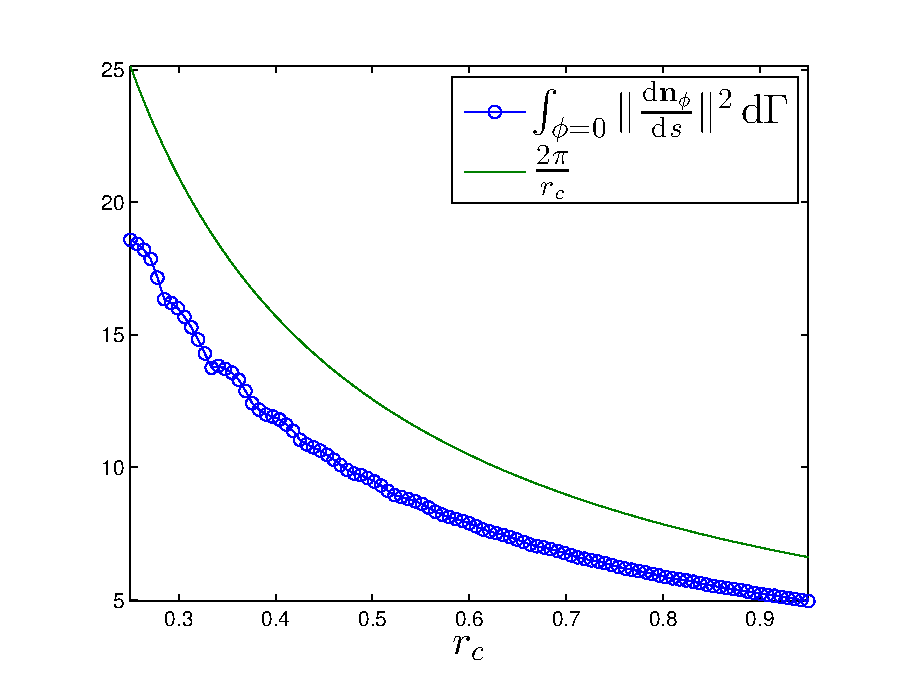
\includegraphics[width=\linewidth]{beam2D_quad4_XFEM_sweep_nphi_InterfaceCurvatureSquared_circle_sol.eps}
		} &
		\subfloat[]{
			\label{fig:beam2D_quad4_XFEM_sweep_nphi_InterfaceCurvatureSquared_circle_error}
			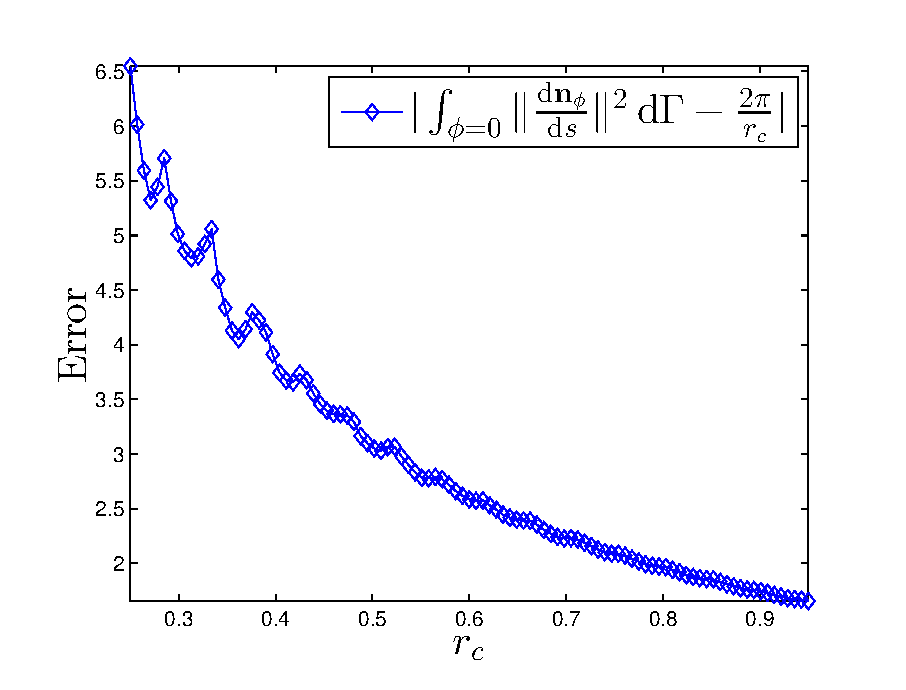
\includegraphics[width=\linewidth]{beam2D_quad4_XFEM_sweep_nphi_InterfaceCurvatureSquared_circle_error.eps}
		}
	\end{tabularx}
	\caption{Squared curvature and absolute error for the circular sweep using the $\mathbf{n}_{\phi}$ formulation, with mesh $45 \times 30$.}
	\label{fig:beam2D_quad4_XFEM_sweep_nphi_InterfaceCurvatureSquared_circle}
\end{figure}
%
The finer mesh results are shown in Figure \ref{fig:beam2D_quad4_XFEM_sweep_nphi_InterfaceCurvatureSquared_circle_finer}.
%
\begin{figure}[H]
	\centering
	\begin{tabularx}{\linewidth}{XX}
		\subfloat[]{
			\label{fig:beam2D_quad4_XFEM_sweep_nphi_InterfaceCurvatureSquared_circle_finer_sol}
			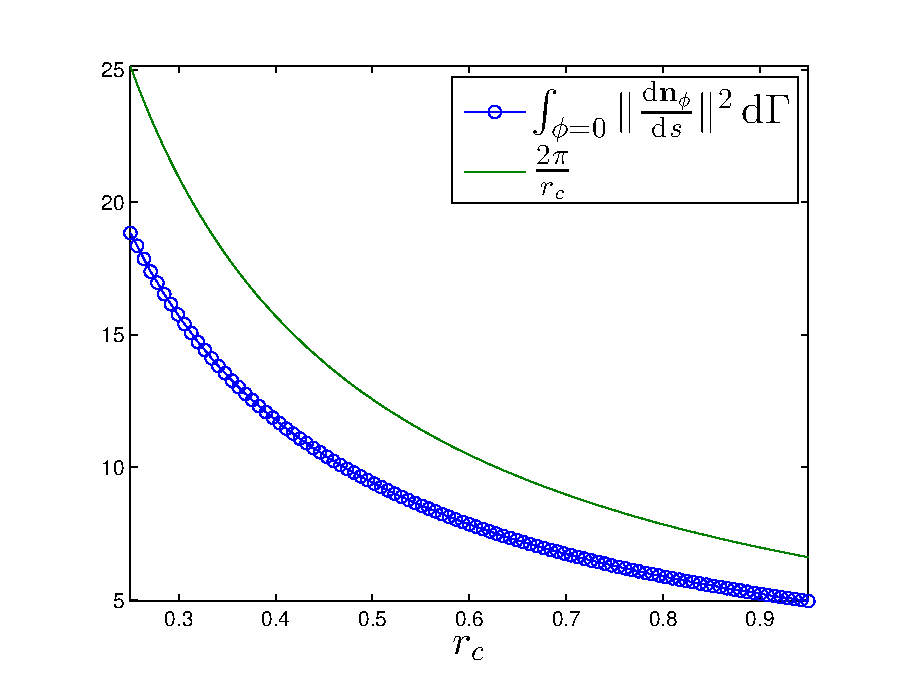
\includegraphics[width=\linewidth]{beam2D_quad4_XFEM_sweep_nphi_InterfaceCurvatureSquared_circle_finer_sol.eps}
		} &
		\subfloat[]{
			\label{fig:beam2D_quad4_XFEM_sweep_nphi_InterfaceCurvatureSquared_circle_finer_error}
			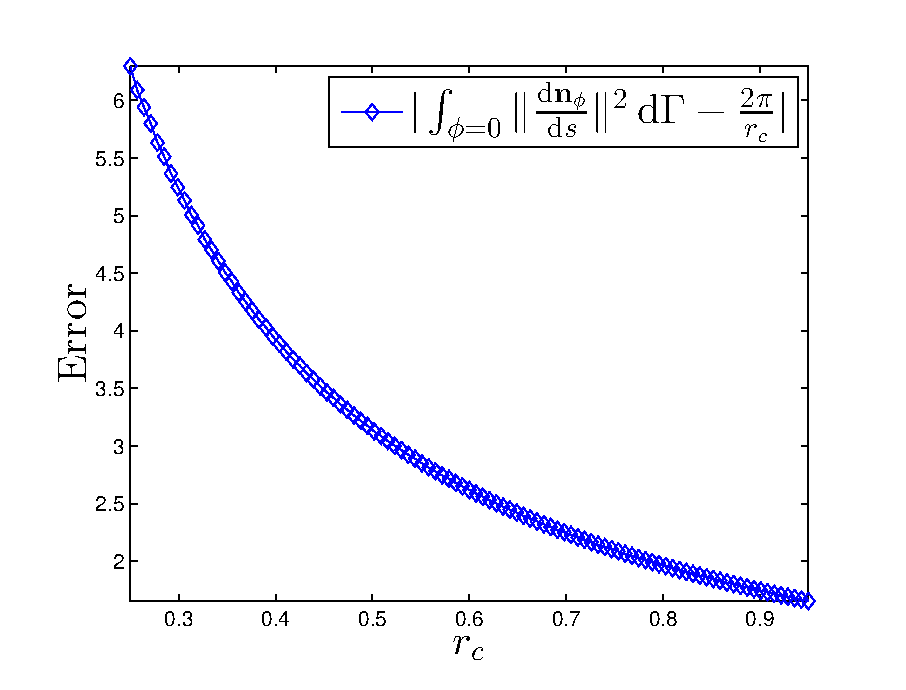
\includegraphics[width=\linewidth]{beam2D_quad4_XFEM_sweep_nphi_InterfaceCurvatureSquared_circle_finer_error.eps}
		}
	\end{tabularx}
	\caption{Squared curvature and absolute error for the circular sweep using the $\mathbf{n}_{\phi}$ formulation, with mesh $180 \times 120$.}
	\label{fig:beam2D_quad4_XFEM_sweep_nphi_InterfaceCurvatureSquared_circle_finer}
\end{figure}
%
% -----------------------------------------------------------------------------

\subsubsection{$\mathbf{n}_{u}$ results}
\label{sec:nnrm_results}

Using the $\mathbf{n}_{u}$ formulation, we get the results displayed in Figures \ref{fig:beam2D_quad4_XFEM_sweep_nnrm_InterfaceCurvatureSquared_circle} and \ref{fig:beam2D_quad4_XFEM_sweep_nnrm_InterfaceCurvatureSquared_sin} for a circle and sinusoidal wave, respectively. The mesh size is $45 \times 30$. The scaling factor, $\gamma_{u}$, is 100.
%
\begin{figure}[H]
	\centering
	\begin{tabularx}{\linewidth}{XX}
		\subfloat[]{
			\label{fig:beam2D_quad4_XFEM_sweep_nnrm_InterfaceCurvatureSquared_circle_sol}
			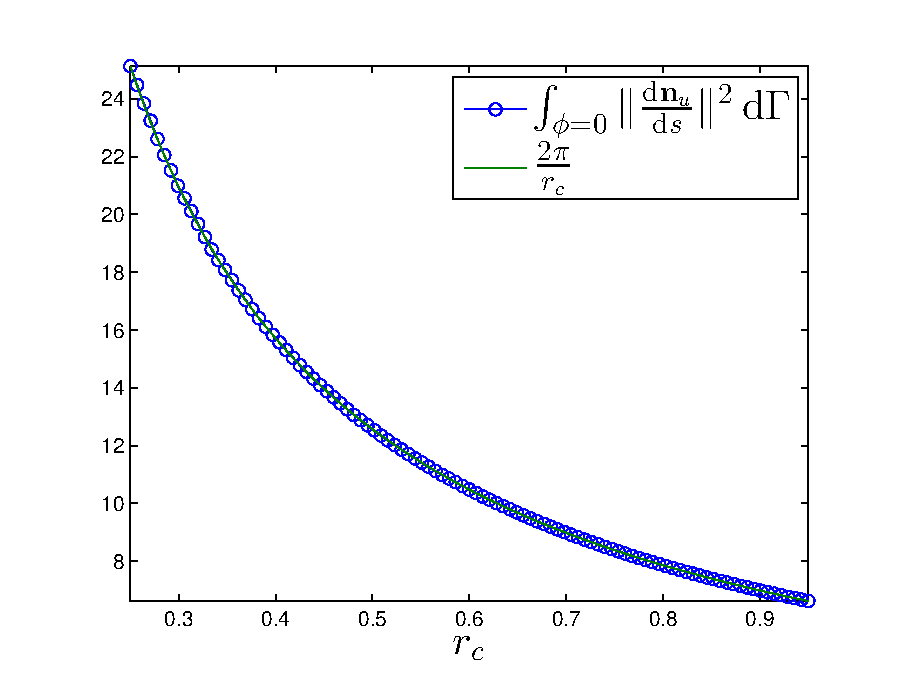
\includegraphics[width=\linewidth]{beam2D_quad4_XFEM_sweep_nnrm_InterfaceCurvatureSquared_circle_sol.eps}
		} &
		\subfloat[]{
			\label{fig:beam2D_quad4_XFEM_sweep_nnrm_InterfaceCurvatureSquared_circle_error}
			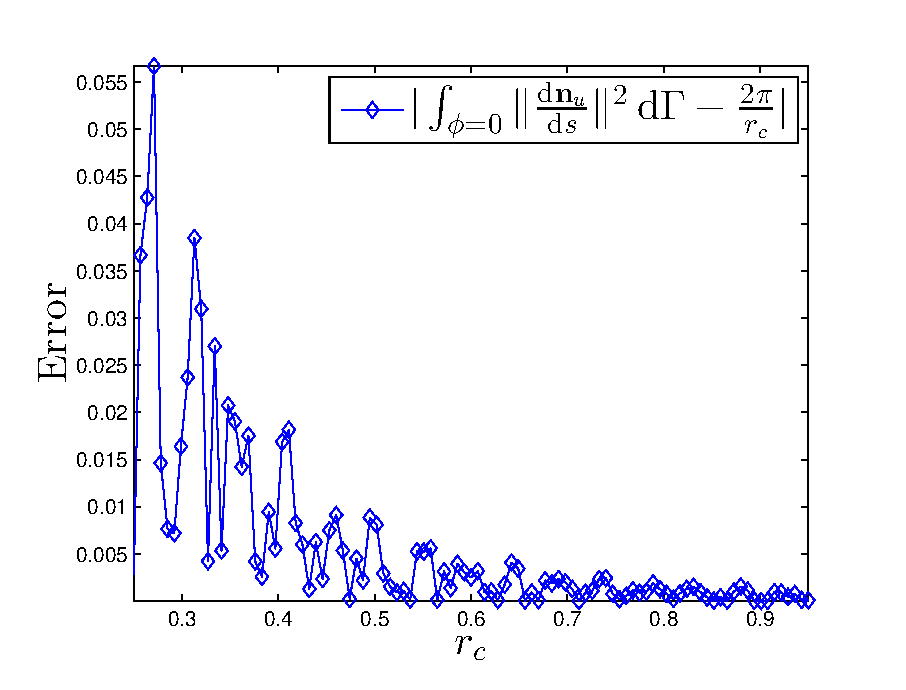
\includegraphics[width=\linewidth]{beam2D_quad4_XFEM_sweep_nnrm_InterfaceCurvatureSquared_circle_error.eps}
		}
	\end{tabularx}
	\caption{Squared curvature and absolute error for the circular sweep using the $\mathbf{n}_{u}$ formulation, with mesh $45 \times 30$.}
	\label{fig:beam2D_quad4_XFEM_sweep_nnrm_InterfaceCurvatureSquared_circle}
\end{figure}
%
\begin{figure}[H]
	\centering
	\begin{tabularx}{\linewidth}{XX}
		\subfloat[]{
			\label{fig:beam2D_quad4_XFEM_sweep_nnrm_InterfaceCurvatureSquared_sin_sol}
			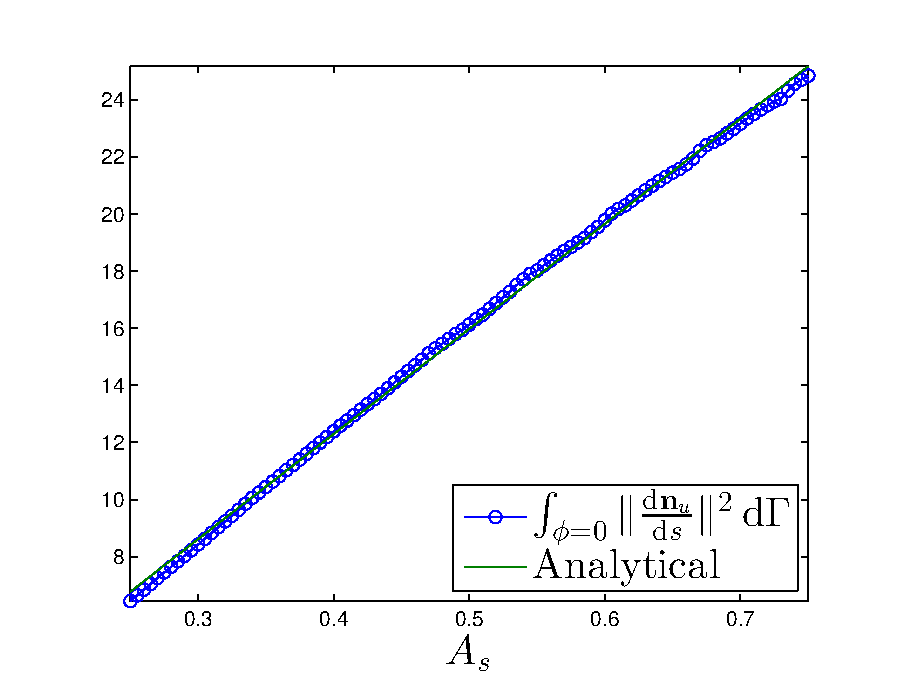
\includegraphics[width=\linewidth]{beam2D_quad4_XFEM_sweep_nnrm_InterfaceCurvatureSquared_sin_sol.eps}
		} &
		\subfloat[]{
			\label{fig:beam2D_quad4_XFEM_sweep_nnrm_InterfaceCurvatureSquared_sin_error}
			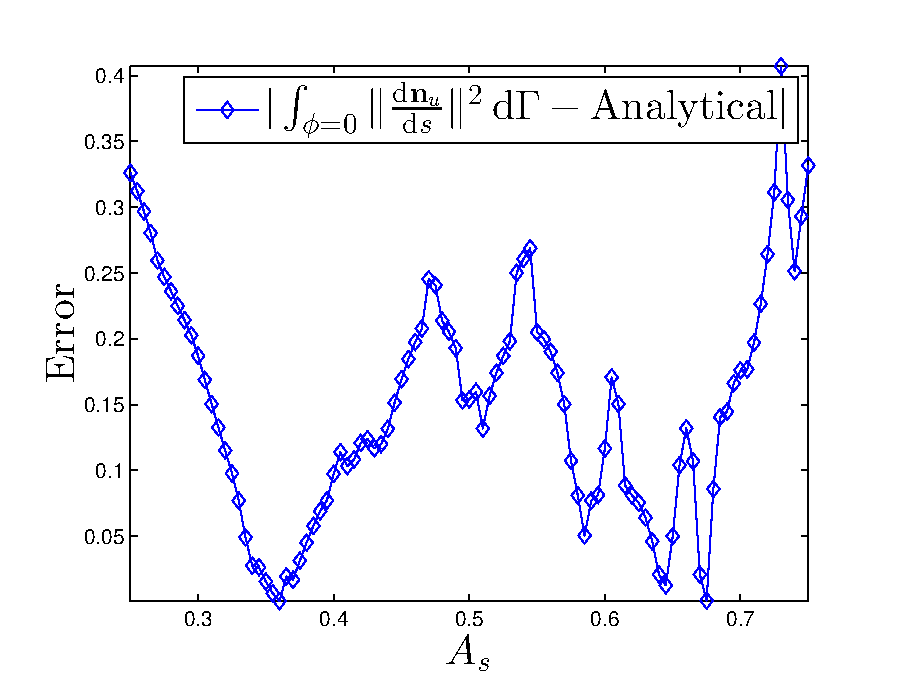
\includegraphics[width=\linewidth]{beam2D_quad4_XFEM_sweep_nnrm_InterfaceCurvatureSquared_sin_error.eps}
		}
	\end{tabularx}
	\caption{Squared curvature and absolute error for the sinusoidal wave sweep using the $\mathbf{n}_{u}$ formulation, with mesh $45 \times 30$.}
	\label{fig:beam2D_quad4_XFEM_sweep_nnrm_InterfaceCurvatureSquared_sin}
\end{figure}
%
% -----------------------------------------------------------------------------

\subsubsection{$\mathbf{n}_{\psi}$ results}
\label{sec:npsi_results}

Measuring the curvature using the $\mathbf{n}_{\psi}$ formulation requires us to define the parameter $\epsilon$. We will examine the influence of $\epsilon = 1.0$, $\epsilon = 2.0$, and $\epsilon = 4.0$, and the benefits of using $\nabla \psi = \frac{\partial \psi}{\partial \mathbf{x}}$ or 
$\nabla \psi = \frac{\partial \psi}{\partial \phi} \frac{\partial \phi}{\partial \mathbf{x}}$.

% -----------------------------------------------------------------------------

\subsubsection{Preliminary conclusions of the sweep study}
\label{sec:sweep_study_conclusions}

Figures \ref{fig:beam2D_quad4_XFEM_sweep_nphi_InterfaceCurvatureSquared_circle} and \ref{fig:beam2D_quad4_XFEM_sweep_nphi_InterfaceCurvatureSquared_circle_finer} show that using $\mathbf{n}_{\phi}$ causes oscillations in the measurement if the mesh is not fine enough. Using a projection scheme in the $\mathbf{n}_{u}$ and $\mathbf{n}_{\psi}$ formulations yields a smoother curvature measure and decreases the error.

% -----------------------------------------------------------------------------
\section{Preliminary optimization results}
\label{sec:optimization_results}

For all the problems studied in this section, we will model a minimal compliance ``solid-void'' structural linear optimization problem:
%
\begin{equation}
	\centering
	\label{eq:curvature_optimization_objective}
	\mathcal{F} = \frac{1}{2} w_{\Pi} \int \boldsymbol{\sigma} : \boldsymbol{\varepsilon} \,\mathrm{d}\Omega^{s} + w_{\kappa} \int_{\phi=0} \kappa_{n} \,\mathrm{d}\Gamma
\end{equation}
%
where the strain energy of the structural problem is computed over the solid phase, $\Omega^{s}$, and $w_{\Pi}$ and $w_{\kappa}$ represent the penalties for the compliance and curvature penalties, respectively. The optimization problem is subject to a volume fraction constraint:
%
\begin{equation}
	\centering
	\label{eq:curvature_optimization_constraint}
	\mathcal{G} = \frac{\int \,\mathrm{d}\Omega^{s}}{\bar{v}_{s}\left(\int \,\mathrm{d}\Omega^{s} + \int \,\mathrm{d}\Omega^{v} \right)} - 1
\end{equation}
%
where $\Omega^{v}$ is the domain of the void region, and $\bar{v}_{s}$ is the maximum volume fraction of the solid phase.

The problem setup is shown in Figure \ref{fig:curvature_opt_setup}. A list of common parameters for all problems is shown in Table \ref{tab:curvature_opt_parameters}.
%
\begin{figure}
	\centering
	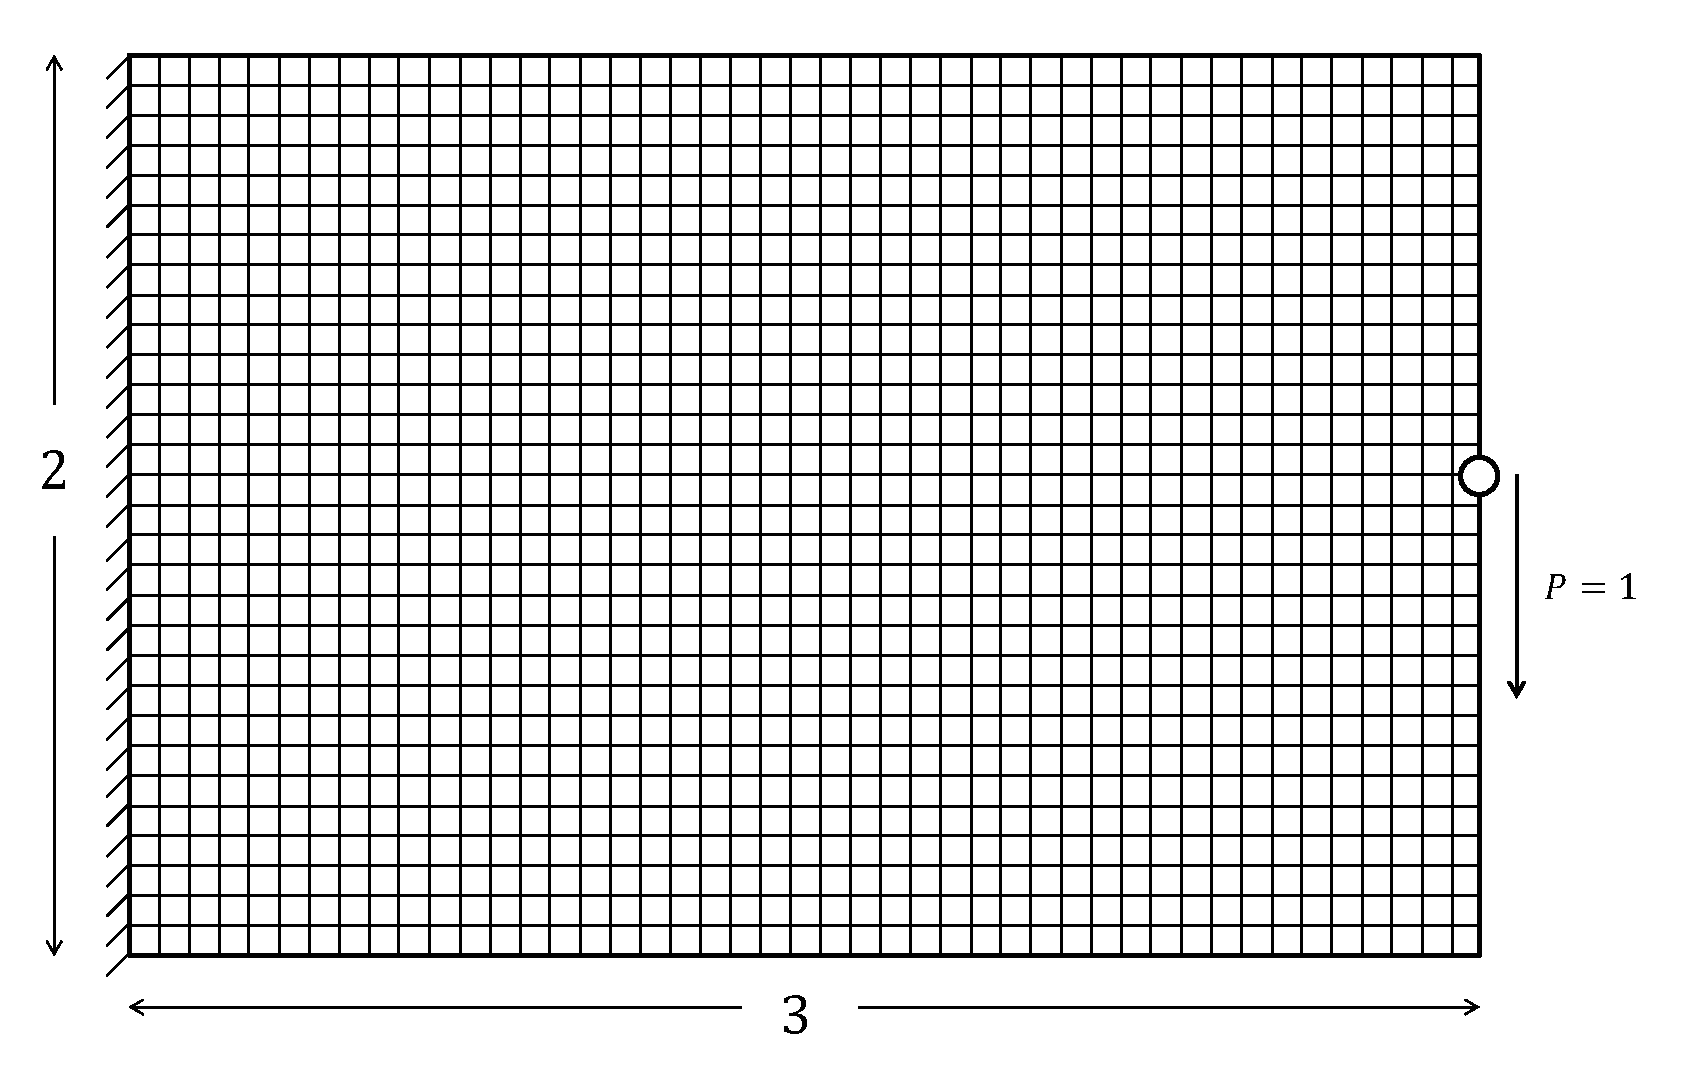
\includegraphics[scale=0.4]{curvature_opt_setup.eps}
	\caption{Setup for the curvature optimization study. A mesh of size $3L \times 2L$, with $45 \times 30$ quadrilateral linear elements is anchored to the wall on its left side, and subject to a point load on its right side.}
	\label{fig:curvature_opt_setup}
\end{figure}
%
\begin{table}
	\centering
	\begin{tabular*}{0.75\textwidth}{l l}
	\hline
	Point load                  & $P = 1$ \\
	Young's modulus             & $E_{xx} = 1$ \\
    Element length              & $h=0.066667$ \\
    Maximum volume fraction     & $\bar{v}_{s} = 0.5$ \\
	Smoothing filter            & $d = 1.6 \cdot h$ \\
	\hline
	\end{tabular*}
	\caption{Parameters for the curvature optimization study.}
	\label{tab:curvature_opt_parameters}
\end{table}
%
The parameters $w_{\Pi}$ and $w_{\kappa}$, and the initial design, will be problem dependent values. For all results, the initial design and its respective level set field will be displayed in the top left corner of the figures.

% -----------------------------------------------------------------------------

\subsection{$\kappa_{n}^2 = \Vert \frac{\mathrm{d}\mathbf{n}_{u}}{\mathrm{d}s}\Vert^2$}

The results for equation \ref{eq:curvature_squared} with formulation $\mathbf{n}_{u}$ are shown in Figures \ref{fig:beam2D_quad4_XFEM_nnrm_InterfaceCurvatureSquared_disp_1.0e+00_curv_1.0e-01} and \ref{fig:beam2D_quad4_XFEM_nnrm_InterfaceCurvatureSquared_disp_1.0e+00_curv_1.0e+00}.
%
\begin{figure}[H]
	\centering
	\includegraphics[scale=0.6]{{beam2D_quad4_XFEM_nnrm_InterfaceCurvatureSquared_disp_1.0e+00_curv_1.0e-01}.eps}
	\caption{Optimized geometry for computing strain energy over the interface \ref{eq:curvature_squared} with formulation $\mathbf{n}_{u}$. $w_{\Pi} = 1$ and $w_{\kappa} = 0.1$. }
	\label{fig:beam2D_quad4_XFEM_nnrm_InterfaceCurvatureSquared_disp_1.0e+00_curv_1.0e-01}
\end{figure}
%
\begin{figure}[H]
	\centering
	\includegraphics[scale=0.6]{{beam2D_quad4_XFEM_nnrm_InterfaceCurvatureSquared_disp_1.0e+00_curv_1.0e+00}.eps}
	\caption{Optimized geometry for computing strain energy over the interface \ref{eq:curvature_squared} with formulation $\mathbf{n}_{u}$. $w_{\Pi} = 1$ and $w_{\kappa} = 1$. }
	\label{fig:beam2D_quad4_XFEM_nnrm_InterfaceCurvatureSquared_disp_1.0e+00_curv_1.0e+00}
\end{figure}
%
% -----------------------------------------------------------------------------

\subsection{$\kappa_{n}^2 = \frac{1}{2} \boldsymbol{\sigma} : \boldsymbol{\varepsilon}$ with $\mathbf{n}_{g}$}

The results for Equation \ref{eq:curvature_strain_energy} with formulation $\mathbf{n}_{g}$ are shown in Figures  \ref{fig:beam2D_quad4_XFEM_beam_lagrange_springs_1.0e-02_search_1.2e+00_disp_1.0e+00_curv_1.0e-01} and \ref{fig:beam2D_quad4_XFEM_beam_lagrange_springs_1.0e-02_search_1.2e+00_disp_1.0e+00_curv_1.0e+00}.
%
\begin{figure}[H]
	\centering
	\includegraphics[scale=0.6]{{beam2D_quad4_XFEM_beam_lagrange_springs_1.0e-02_search_1.2e+00_disp_1.0e+00_curv_1.0e-01}.eps}
	\caption{Optimized geometry for computing strain energy over the interface \ref{eq:curvature_strain_energy} with formulation $\mathbf{n}_{g}$. $w_{\Pi} = 1$ and $w_{\kappa} = 0.1$. $k_{\kappa} = 0.01$ and $r_{\kappa} = 1.2$. }
	\label{fig:beam2D_quad4_XFEM_beam_lagrange_springs_1.0e-02_search_1.2e+00_disp_1.0e+00_curv_1.0e-01}
\end{figure}
%
\begin{figure}[H]
	\centering
	\includegraphics[scale=0.6]{{beam2D_quad4_XFEM_beam_lagrange_springs_1.0e-02_search_1.2e+00_disp_1.0e+00_curv_1.0e+00}.eps}
	\caption{Optimized geometry for computing strain energy over the interface \ref{eq:curvature_strain_energy} with formulation $\mathbf{n}_{g}$. $w_{\Pi} = 1$ and $w_{\kappa} = 1$. $k_{\kappa} = 0.01$ and $r_{\kappa} = 1.2$. }
	\label{fig:beam2D_quad4_XFEM_beam_lagrange_springs_1.0e-02_search_1.2e+00_disp_1.0e+00_curv_1.0e+00}
\end{figure}
%
% -----------------------------------------------------------------------------

\section{Conclusions}
\label{sec:curvature_conclusions}

Measuring curvature as a function of the level set unit normal yields results that are not smooth at the points where the level set function cuts the elements. Equating curvature to strain energy and measuring its value at the points of intersection yields smoother results, at the cost of increased sensitivity. However, inserting a field of artificial springs to allow for the points to displace reduces the sensitivities and yields smoother optimized geometries.

The author plans to finalize the sweep with $\mathbf{n}_{\psi}$ and $\mathbf{n}_{g}$ and perform further optimization runs.

% -----------------------------------------------------------------------------
% Acknowledgement

% \subsection*{Acknowledgement}
% 
% The authors acknowledge the support of the National Science Foundation under grant EFRI-ODISSEI  1240374 and CBET 1246854. The opinions and conclusions presented in this paper are those of the authors and do not necessarily reflect the views of the sponsoring organization.

% -----------------------------------------------------------------------------
% Bibliography

% \bibliographystyle{etc/spbasic}
% \bibliography{etc/JabRefDatabase}

% \end{document}
